%%%%%%%%%%%%%%%%%%%%%%%%%%%%%%%%%%%%%%%%%%%%%%%%%%%%%%%%%%%%%%%%%%%%%%%%%%%%
%    This LaTeX source was automatically generated by outlinebeamer.pl     %
%                                                                          %
%   Remember that most changes should be made to the outline source file   %
% changes to this file will be overwritten when the file gets regenerated  %
%                                                                          %
%                  outlinebeamer - Outline Beamer Class Presentation Maker %
%                                    http://outlinebeamer.sourceforge.net/ %
%%%%%%%%%%%%%%%%%%%%%%%%%%%%%%%%%%%%%%%%%%%%%%%%%%%%%%%%%%%%%%%%%%%%%%%%%%%%
%\documentclass{beamer}
\documentclass{beamer}

\usetheme{Copenhagen}
\usecolortheme{default}

\newcommand{\Code}[1]{\textsf{#1}}
\newcommand{\cello}{\textsf{Cello}}
\newcommand{\enzo}{\textsf{Enzo}}
\newcommand{\code}[1]{\texttt{#1}}
\newcommand{\us}[1]{\color{blue}{#1}}
\newcommand{\them}[1]{\color{red}{#1}}
\newcommand{\newus}[1]{\color{magenta}{#1}}
\newcommand{\good}{\textcolor{green}{\smiley}}
\newcommand{\bad}{\textcolor{red}{\frownie}}
\newcommand{\colorcode}[1]{\textcolor{blue}{\code{#1}}}
\newcommand{\itemnum}[1]{\item<#1>}

% UNCOMMENT TO PRINT

% \newcommand{\enhance}[1]{}
% \newcommand{\enhancebf}[2]{\textbf{#2}}
% \newcommand{\enhanceus}[1]{\color{blue}}
% \newcommand{\enhancenewus}[1]{\color{magenta}}
% \newcommand{\enhancethem}[1]{\color{red}}

% UNCOMMENT FOR TALK:

\newcommand{\enhance}[1]{\temporal<#1>{\color{lightgray}}{\color{black}}{\color{gray}}}
\newcommand{\enhancebf}[2]{\enhance{#1}\textbf{#2}}
\newcommand{\enhanceus}[1]{\temporal<#1>{\color{lightgray}}{\color{blue}}{\color{blue}}}
\newcommand{\enhancenewus}[1]{\temporal<#1>{\color{lightgray}}{\color{magenta}}{\color{magenta}}}
\newcommand{\enhancethem}[1]{\temporal<#1>{\color{lightgray}}{\color{red}}{\color{red}}}



% \def\enhanceus<#1>{%
%  \temporal<#1>{\color{lightgray}}{\color{blue}}{\color{blue}}}
% \def\enhancenewus<#1>{%
%  \temporal<#1>{\color{lightgray}}{\color{magenta}}{\color{magenta}}}
% \def\enhancethem<#1>{%
%  \temporal<#1>{\color{lightgray}}{\color{red}}{\color{red}}}

\newcommand{\ENHANCE}[1]{
 \temporal<#1>{\color{lightgray}}{\color{black}}{\color{gray}}}

%\includeonly{array-amr}


%======================================================================
\title[The \cello\ Project]
      {The \cello\ Project \\ \small{\enzo: The Next Generation}}
\author[James Bordner]{\small Laboratory for Computational Astrophysics \\ Center for Astrophysics and Space Sciences \\San Diego Supercomputer Center \\ University of California, San Diego \\ \ \\ James Bordner}
\date{\today}
\begin{document}
\frame{\titlepage}
%\frame{\tableofcontents}
% \AtBeginSubsection[]
{
%------------------------------------------------------------------------
%  \begin{frame}<beamer>
%    \tableofcontents[currentsection,currentsubsection]
%    \tableofcontents[currentsection]
%  \end{frame}
}

%========================================================================
\section{Introduction}
%========================================================================

% \include{outline}

%------------------------------------------------------------------------
\subsection{Goals}
%------------------------------------------------------------------------
\begin{frame}[fragile] \frametitle{Project Goals}
   \begin{itemize}
      \item\enhance{1} \enzo: The Next Generation
      \item\enhance{2} Computational astrophysics code for next 10+ years
      \item\enhance{3} Scalable to largest available platforms: O($10^{5+}$)  cores
      \item\enhance{4} Easy modify, enhance, adapt, maintain
      \item\enhance{5} Easy to define and run new problems
      \enhance{6}\item Capable of advancing science knowledge
   \end{itemize}
\end{frame}



%------------------------------------------------------------------------
\subsection{Scope}
%------------------------------------------------------------------------

%------------------------------------------------------------------------
    \begin{frame}[fragile] \frametitle{Target Classes of Users}
      \begin{itemize}
        \item \enhancebf{1}{Graduate students}
        \begin{itemize}
          \item \enhance{1}easy to define problem, run, and analyze
          \item \enhance{1}minimal software-, hardware-, or method-related ``gotcha's''
        \end{itemize}
        \item \enhancebf{2}{Physics experts}
        \begin{itemize}
          \item \enhance{2}deep control of physics parameters
          \item \enhance{2}ability to solve a wide range of problems
        \end{itemize}
        \item \enhancebf{3}{Numerical experts}
        \begin{itemize}
          \item \enhance{3}deep control of method parameters
          \item \enhance{3}easy to incorporate new methods
        \end{itemize}
        \item \enhancebf{4}{Computing experts}
        \begin{itemize}
          \item \enhance{4}deep control of data structures
          \item \enhance{4}AMR, parallelization, data distribution, array layout
        \end{itemize}
      \end{itemize}
\end{frame}

%------------------------------------------------------------------------
    \begin{frame}[fragile] \frametitle{Target Classes of Problems}

      \begin{itemize}
        \item \enhance{1}\textbf{Unigrid (turbulence)}
        \begin{itemize}
          \item  \enhance{1}parallelizes fully
          \item  \enhance{1}\enzo\ does well, but still room for improvement
        \end{itemize}
        \item \enhance{2}\textbf{``Typical'' AMR (cosmology)}
        \begin{itemize}
	   \item \enhance{2}\enzo\ does ok, but has scaling issues
	   \item \enhance{2}load-balancing, memory usage, etc.
        \end{itemize}
        \item \enhance{3}\textbf{``Deep'' AMR (star formation)}
        \begin{itemize}
          \item \enhance{3}most difficult to parallelize effectively
          \item \enhance{3}\enzo\ has done deep runs, but not without difficulty
          \item \enhance{3}floating-point precision and integer range issues
        \end{itemize}
        \item \enhance{4}\textbf{Ensembles (parameter studies)}
        \begin{itemize}
           \item \enhance{4}Inter-simulation inline analysis
        \end{itemize}
 
      \end{itemize}
\end{frame}



%------------------------------------------------------------------------
\subsection{Issues}
%------------------------------------------------------------------------

%------------------------------------------------------------------------
\begin{frame}[fragile] \frametitle{Petascale performance Issues}
   \begin{itemize}
      \item \enhance{1}Parallel task control
      \begin{itemize}
          \item \enhance{1}Large enough to be efficient
          \item \enhance{1}Small enough for sufficient parallelism
      \end{itemize}
      \item \enhance{2}Parallel task scheduling
      \begin{itemize}
          \item \enhance{2}Static scheduling with dynamic load balancing
          \item \enhance{2}Dynamic scheduling with job migration
      \end{itemize}
      \item \enhance{3}Load balancing across nodes / cpus / cores
      \item \enhance{4}Global synchronization
      \item \enhance{5}Software resiliency / fault tolerance
      \item \enhance{6}Checkpoint / restart
   \end{itemize}
\end{frame}


%========================================================================
\section{Software design}
%========================================================================

%------------------------------------------------------------------------
\subsection{Input files}
%------------------------------------------------------------------------

\begin{frame}[fragile] \frametitle{Input Files}
\begin{itemize}
   \item\enhance{1}Important: point-of-contact between user and application
   \item\enhance{2}Limiting factor in usability and power of the application
   \item\enhance{3}Maximize expressibility while minimizing complexity
   \item\enhance{4}Approach: remove ``\code{ProblemType}'' parameter
   \begin{itemize}
      \item\enhance{5}Restricts scope of problems solved
      \item\enhance{6}Overall code size will be much smaller
   \begin{itemize}
      \item\enhance{7} \code{19.8\%} of \enzo\ C++ functions contain ``Initialize''!
   \end{itemize}
      \item\enhance{8}Can fake it with e.g.~\code{\#include "implosion.param"}
   \end{itemize}
\end{itemize}
\end{frame}

\begin{frame}[fragile] \frametitle{Input Files}
\begin{itemize}
   \item\enhance{1}Helpful to have more powerful syntax and grammar
  \begin{block}{}\footnotesize\enhance{2}
      \verb+Method ppm {+ \\
      \verb+   diffusion = false;+ \\
      \verb+}+
   \end{block}
   \item\enhance{3}Requires more data types
  \begin{block}{}\footnotesize
  \begin{tabular}{ll}
	\enhance{4}Scalar expressions &\enhance{4} \code{exp(cos(x) + sin(y))} \\
	\enhance{4}Logical expressions &\enhance{4} \code{x*x + y*y <= 1} \\
       \enhance{4} Lists  &\enhance{4} \code{[1.9e6, x <= y, "wtf"]}
   \end{tabular}
   \end{block}
   \item\enhance{5} Input file parsing not overly difficult
   \begin{itemize}
      \item\enhance{5} \code{flex} and \code{bison} tools
   \end{itemize}
\end{itemize}
\end{frame}

\include{implosion-1}
%------------------------------------------------------------------------
\begin{frame}[fragile] \frametitle{Draft Input File: Implosion}
\footnotesize
\begin{block}{Implosion: method parameters and boundary conditions}
\begin{verbatim}
# PPM hydrodynamics

Method ppm {
   gamma     = 1.4;
   courant   = 0.8;
   diffusion = true;
   flattening = true;
   steepening = true;
}

# Define boundary conditions

Boundary { type = "reflecting" }
\end{verbatim}
\end{block}
\end{frame}

\include{implosion-3}

%------------------------------------------------------------------------
\subsection{Software components}
%------------------------------------------------------------------------

%@@@@@@@@@@@@@@@@@@@@@@@@@@@@@@@@@@@@@@@@@@@@@@@@@@@@@@@@@@@@@@@@@@@@@@@
\chapter{Components} \label{c:components}
%@@@@@@@@@@@@@@@@@@@@@@@@@@@@@@@@@@@@@@@@@@@@@@@@@@@@@@@@@@@@@@@@@@@@@@@

% \centerline{\includegraphics{uml/core-components.1}}


\centerline{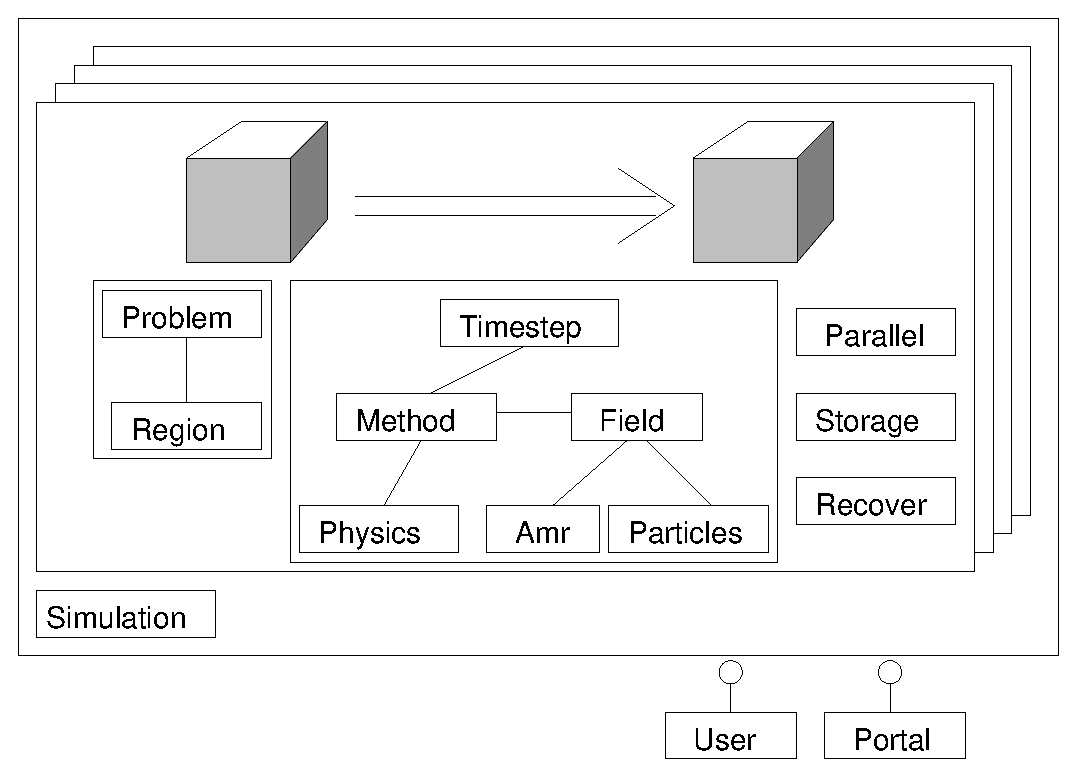
\includegraphics[totalheight=3in]{components.eps}}

   This chapter describes the design of \cello\ at the component
   level.  Each component is described, including the component
   interdependencies, interface, and classes.

\begin{description}
%
 \item [Simulation (\S\ref{s:component-simulation}): ]
%
        Description and management of computational astrophysics
        problem or ensemble of problems.  Controls sequencing of and
        interactions between other components such as \code{Parallel},
        \code{Method}, and \code{Field}.
%
 \item [Problem (\S\ref{s:component-problem}): ]
%
        The problem refers to the initial setup of the problem,
        including the domain, boundary and initial conditions.
%
 \item [Region (\S\ref{s:component-region}): ]
%
        A \code{Region} is a portion of space and time.
        \code{Region}s are used whenever problem characteristics, data
        structure behavior, or physics computations vary between
        different spacial or temporal \code{Region}s.  A \code{Region}
        is used to define the entire domain.  \code{Region}s may vary
        in time, for example they may grow, shrink, appear, or
        disappear.
%
 \item [Timestep (\S\ref{s:component-timestep}): ]
%
        \code{Timestep} handles the timestepping of methods to advance
        the problem forward in time.
%
 \item [Method (\S\ref{s:component-method}): ]
%
        Defines how to simulate the physics in the computational
        universe.  A \code{Method} specifies the numerical method to
        use, which \code{Field}s are involved, and any associated
        method-specific parameters.  Sequencing and coupling of
        \code{Method}s is defined in \code{Problem} and implemented in
        \code{Control}.  Analysis and visualization are considered
        \code{Method}s as well.
%
 \item [Physics (\S\ref{s:component-physics}): ]
%
        Defines what physics to simulate in the computational
        universe.  Used to define which physics processes are enabled,
        such as self-gravity, hydrodynamics, cosmological expansion,
        etc.  Also defines any parameters associated with the physics
        of the problem being solved, such as cosmological parameters
        and the gravitational constant.
%
 \item [Field (\S\ref{s:component-field}): ]
%
        A \code{Field} is used to represent a specific continuous
        scalar or vector field.  The actual \code{Field} is
        represented either using adaptive mesh refinement via
        \code{Amr}, or as a collection of particles using
        \code{Particles}.  Includes \code{Units} to define the problem
        units, as well as scaling amount to improve numerics, and
        scaling quantization to avoid precision loss.
%
 \item [Amr (\S\ref{s:component-amr}): ]
%
        The \code{Amr} component includes classes for representing
        multi-resolution data on a hierarchy of grid patches of
        varying spacial and temporal resolutions.  The \code{AMR} data
        structures can have multiple levels of data distribution and
        parallelism.  Uses the \code{Parallel} component for
        controlling the parallel communication, synchronization, and
        load-balancing.
%
 \item [Particles (\S\ref{s:component-particles}): ]
%
        The \code{Particles} component serves to represent multi-level
        parallel distribution of sets of various types of particle
        data.  Uses the \code{Parallel} component for controlling the
        parallel communication, synchronization, distribution, and
        load-balancing of \code{Particles}.
%
 \item [Array (\S\ref{s:component-array}): ]
%
        The \code{Array} component is used for representing a single
        array of up to $3$ dimensions.  The \code{Array} may include
        options for MPI-, OMP-, UPC-, or GPU-based parallelism, as
        well as options for controlling memory layout to improve cache
        performance.
%
 \item [Parallel (\S\ref{s:component-parallel}): ]
%
        The \code{Parallel} component is used to specify and control
        the levels of parallelizion (simulations, patches, and
        subblocks), type of parallelization (shared- or
        distributed-memory), and mechanism for controling the
        parallelism (MPI-1 2-sided, MPI-2 1-sided, OpenMP, UPC).
        Lower-level parameters provide detailed control of buffering,
        blocking or nonblocking, patch-to-processor mapping,
        subblock-to-thread mapping, etc.
%
 \item [Disk (\S\ref{s:component-disk}): ]
%
        The \code{Disk} component controls what, when, and how to
        input and output large-scale data to long-term permanent
        storage, primarily \code{Fields} (represented as
        \code{Particles} or \code{Arrays}).
%
 \item [Memory (\S\ref{s:component-memory}): ]
%
        The \code{Memory} component controls dynamic memory
        allocation, and includes features for monitoring memory usage,
        improving performance, and verifying correctness.
%
 \item [Error (\S\ref{s:component-error}): ]
%
        The \code{Error} package is used to detect errors, evaluate
        them, and decide what to do about them.  This includes
        maintaining restart data dumps, and may involve shutting down
        a processor or node and rebalancing the data, etc.
%
 \item [Parameters (\S\ref{s:component-parameters}): ]
%
        The \code{Parameters} component
        reads in a parameter file or files, and provides the
        application access to parameter values.
%
%
 \item [Performance (\S\ref{s:component-performance}): ]
%
        The \code{Performance} component monitors performance such as
        memory usage, computation amount, parallel communication,
        parallel load balancing, disk storage, etc., and provides
        access functions to be called from other components.
%
 \item [Monitor (\S\ref{s:component-monitor}): ]
%
        The \code{Monitor} component controls what and when to output
        user-readable summary information about the running
        application, such as status summary, progress, warnings,
        errors, and performance information.
%
 \item [Portal (\S\ref{s:component-portal}): ]
%
        The \code{Portal} component controls the interaction of the
        application with external applications, for both obtaining
        information about a running simulation, and controling it.
\end{description}

%-----------------------------------------------------------------------

%=======================================================================
\section{\code{Simulation} Component} \label{s:component-simulation}
%=======================================================================

Given \code{Physics}, \code{Methods}, and \code{Amr} or
\code{Particles} data structures, specifies and implements the
top-level sequencing and properties of the \code{Problem} (or
\code{Problems} in the case of an ensemble) to run.

\begin{itemize}
\item \code{Simulation}
\item \code{Ensemble}
\item \code{Control}
\item \code{Problem}
\item \code{Physics}
\item \code{Method}
\item \code{IO}
\end{itemize}

\subsection{Attributes.}

\subsection{Operations}

%=======================================================================
\subsection{\code{Ensemble} Component} \label{s:component-ensemble}
%=======================================================================

The \code{Ensemble} class is used to define a ensemble of simulations.  

\subsection{Attributes.}

\subsection{Operations}


%=======================================================================
\subsection{Control Component} \label{ss:component-control}
%=======================================================================


Global simulation control.

Output types and parameters

\begin{itemize}
\item checkpoint (dump all)
\item output (specific fields)
\item movies (type and rate)
\item analysis (type of analysis, rate)
\item level of output (files for timestep, time, etc.)
\end{itemize}

%-----------------------------------------------------------------------
\subsection{Use Cases}
%-----------------------------------------------------------------------
%-----------------------------------------------------------------------
\subsection{Parameters}
%-----------------------------------------------------------------------

Problem parameters specify the setup of the physical problem,
including initial conditions of relevant data fields and boundary
conditions.

  dimensionality
  domain extents
  initial conditions (materials, subregions, input)
 boundary conditions (periodic, in-/out-flow, specified, dynamic)

Problem parameters include initial conditions and boundary conditions.

Different types of boundary conditions are supported, including
periodic, in- and out-flow, specified, and dynamic.  Different
boundary conditions can be specified for the entire domain, on
separate faces, on subregions of faces, or on specific zones.
Different boundary conditions can be specified for different fields.
%-----------------------------------------------------------------------
\subsection{Use Cases}
%-----------------------------------------------------------------------

\begin{verbatim}
   problem {
      boundary {
         x:lower = reflecting
         x:upper = { type = reflecting }
         y       = { type = periodic }
         z       = { type = inflow,  value = 1.0 }
         z       = { outflow, 1.0 }
      }
   }
\end{verbatim}

\begin{verbatim}
   XM = boundary { x = domain:lower[0] }
   XP = boundary { x = domain:upper[0] }
   YM = boundary { y = domain:lower[1] }
   YP = boundary { y = domain:upper[1] }
   ZM = boundary { z = domain:lower[2] }
   ZP = boundary { z = domain:upper[2] }
   field {
      name = "density"
      value(XM) = 0
      value(XP) = 0
      value(YM) = value (YP)
      value(ZM) = +t
      value(ZM) = -t
   }
\end{verbatim}

%=======================================================================
\subsection{Domain} \label{ss:component-domain}
%=======================================================================

The \code{domain} function is used to specify properties of the
domain.  Domains are boxes aligned with the axes of the computational
coordinate system, and are uniquely determined by the spacial
dimension, and the lowest and highest points in the domain.

%-----------------------------------------------------------------------
\subsubsection{Use Cases}
%-----------------------------------------------------------------------

\begin{verbatim}
   domain { 
      dimension = 3
      lower     = <-3e9,-3e9,-3e9>
      upper     = <3e9,3e9,3e9>
   }
\end{verbatim}

\begin{verbatim}
   domain { 3, <-3e9,-3e9,-3e9>, <3e9,3e9,3e9> }  // Implicit ordering
\end{verbatim}

\begin{verbatim}
   domain { 
      dimension = 3
      upper     = 3e9        // expand scalar to vector
      lower     = -upper     // parameters can be accessed as values
   }
\end{verbatim}

Include errors.

%-----------------------------------------------------------------------
\subsubsection{Parameters}
%-----------------------------------------------------------------------

 \todo\ \textit{Decide: allow defaults?  allow optional parameters?  Special
 \code{OPT\_} prefix for optional parameters?  Write out explicit copy
 of input file?}

The \code{domain} function has three parameters

\begin{tabular}{lll} \\
Name & Type & Restrictions \\ \hline
\code{dimension} & Scalar & $1-3$ \\
\code{lower}     & Vector & length = \code{dimension} \\
\code{upper}     & Vector & length = \code{dimension}, \code{upper} $>$ \code{lower}
\end{tabular}

Lower and upper points are given in units given by \code{units},
described in \S\ref{ss:params-units}.

%-----------------------------------------------------------------------
\subsubsection{Restrictions}
%-----------------------------------------------------------------------

\begin{enumerate}
\item The dimension must be 1, 2, or 3.
\item The number of coordinates in both lower and upper points must equal the dimension.
\item Each coordinate of the lower point must be strictly greater than the corresponding coordinate of the upper point.
\end{enumerate}


%-----------------------------------------------------------------------
\subsubsection{Parameters}
%-----------------------------------------------------------------------

%-----------------------------------------------------------------------
\subsection{\code{Boundary}} \label{ss:component-boundary}
%-----------------------------------------------------------------------

The \code{Boundary} class is used to define the boundary conditions on
the domain.

%-----------------------------------------------------------------------
\subsection{\code{Initial}} \label{s:component-initial}
%-----------------------------------------------------------------------

The \code{Initial} class is used to define the initial conditions for
a problem.




%=======================================================================
\section{Problem parameters} \label{s:problem}
%=======================================================================

Problem parameters include initial conditions and boundary conditions.

Different types of boundary conditions are supported, including
periodic, in- and out-flow, specified, and dynamic.  Different
boundary conditions can be specified for the entire domain, on
separate faces, on subregions of faces, or on specific zones.
Different boundary conditions can be specified for different fields.
%-----------------------------------------------------------------------
\subsection{Use Cases}
%-----------------------------------------------------------------------

\begin{verbatim}
   problem {
      boundary {
         x:lower = reflecting
         x:upper = { type = reflecting }
         y       = { type = periodic }
         z       = { type = inflow,  value = 1.0 }
         z       = { outflow, 1.0 }
      }
   }
\end{verbatim}

\begin{verbatim}
   XM = boundary { x = domain:lower[0] }
   XP = boundary { x = domain:upper[0] }
   YM = boundary { y = domain:lower[1] }
   YP = boundary { y = domain:upper[1] }
   ZM = boundary { z = domain:lower[2] }
   ZP = boundary { z = domain:upper[2] }
   field {
      name = "density"
      value(XM) = 0
      value(XP) = 0
      value(YM) = value (YP)
      value(ZM) = +t
      value(ZM) = -t
   }
\end{verbatim}

%-----------------------------------------------------------------------
\subsection{Parameters}
%-----------------------------------------------------------------------


%=======================================================================
\section{Region Component} \label{s:component-region}
%=======================================================================

Specify partitions of the domain into regions.  Each region contains
different materials with different properties.  Example partitions may
be half-planes, spheres, boxes, or specified using a file containing a
zone bit mask.  Default is region 0, first region is region 1, etc.
Use solid modeling representations?

%-----------------------------------------------------------------------
\subsection{Use Cases}
%-----------------------------------------------------------------------

\begin{verbatim}
   region {
      x + y + z < 0.5
   }
\end{verbatim}

\begin{verbatim}
   BOX = region {
      (x > 0) &&
      (x < 1) &&
      (y > 0) && (y < 1) &&
      (z > 0) && (z < 1)
   }
\end{verbatim}

\begin{verbatim}
   region {
      union {
         region {BOX, translate = 0.0*x, scale = 0.1}
         region {BOX, translate = 0.1*x, scale = <0.1,0.1,0.1>}
         region {BOX, translate = 0.2*x, scale = 0.1}
      }
   }
\end{verbatim}

\begin{verbatim}
   region {
      x = domain:lower[0]
   }
\end{verbatim}

\begin{verbatim}
   region {
      x*x + y*y + z*z < 1
   }
\end{verbatim}

\begin{verbatim}
   region {
      bitmask = "filename.hdf5"
   }
\end{verbatim}


%-----------------------------------------------------------------------
\subsection{Parameters}%
-----------------------------------------------------------------------


%=======================================================================
\section{Timestep Component} \label{s:component-timestep}
%=======================================================================

Global simulation timestepping.

Output types and parameters


%=======================================================================
\section{Method parameters} \label{s:method}
%=======================================================================

 Specify the algorithms and algorithm parameters
 to use for each physics component.  Each physics component has a
 default; some components may have only one available
 (e.g.~cosmological expansion).  Algorithms is in the solution domain.

\begin{itemize}
\item PPM hydro (dual-energy, etc.)
\item gravity solver (FAC, smoother, levels, etc.)
\end{itemize}

%-----------------------------------------------------------------------
\subsection{Use Cases}
%-----------------------------------------------------------------------
%-----------------------------------------------------------------------
\subsection{Parameters}
%-----------------------------------------------------------------------



%=======================================================================
\section{Physics Component} \label{s:component-physics}
%=======================================================================

   Defines what physics to simulate in the computational universe.
   Used to define which physics processes are enabled, such as
   self-gravity, hydrodynamics, cosmological expansion, etc.  Also
   defines any parameters associated with the physics of the problem
   being solved, such as cosmological parameters and the gravitational
   constant.


 matter
 hydrodynamics
  cosmological expansion
 self-gravity

Hydrodynamics


Specify physics modules and physics parameters, including
hydrodynamics, self-gravity, gravitational constant, imposed gravity,
chemistry, cosmological expansion, star formation, etc.  Physics is in
the problem domain.

Specify physics components

\begin{itemize}
\item hydrodynamics
\item  cosmological expansion
\item self-gravity
\end{itemize}

%-----------------------------------------------------------------------
\subsection{Use Cases}
%-----------------------------------------------------------------------
%-----------------------------------------------------------------------
\subsection{Parameters}
%-----------------------------------------------------------------------

%=======================================================================
\subsection{Matter Component} \label{ss:component-matter}
%=======================================================================

 Matter defines properties of matter, such as the matter type (baryonic
 or dark matter), and gas constants.

%-----------------------------------------------------------------------
\subsection{Use Cases}
%-----------------------------------------------------------------------

\begin{verbatim}
   Matter {
      type = dark
   }
\end{verbatim}

\begin{verbatim}
   Matter {
      type  = gas_ideal
      gamma = 1.4
      region { (x < 0) || (x > 1) }
   }
\end{verbatim}

%=======================================================================
\section{Field parameters} \label{s:field}
%=======================================================================

Scalar and vector fields for each material, such as
 density, energy, velocity, etc.  [Merge with Materials?]  Specify
 values, or input from files.

%-----------------------------------------------------------------------
\subsection{Use Cases}
%-----------------------------------------------------------------------
\begin{verbatim}
   field {
      name     = "density"
      name     = "rho"
      type     = scalar
      location = center
   }
   field {
      name     = "velocity"
      name     = "u"
      type     = vector
      location = center
   }
   field {
      name     = "temperature"
      name     = "T"
      type     = scalar
      location = center
   }
   field {
      name     = "B"
      type     = computed
      location = face
   }
\end{verbatim}
%-----------------------------------------------------------------------
\subsection{Parameters}
%-----------------------------------------------------------------------

%=======================================================================
\section{AMR Component} \label{s:component-amr}
%=======================================================================

The \code{Amr} component defines the data structures and associated
parameters for the ``inter-resolution'' aspect of data fields on
distributed AMR hierarchies.  The ``intra-resolution'' aspects are
defined using the closely related \code{Array} component.  Both
patch-based AMR, ala \enzo, and octree-like-based AMR datastructures
are supported.  Support for associating \code{Particle} groups with
\code{Array}'s in an \code{Amr} hierarchy is also included in the
\code{Amr} component.

Tentative features of \code{Amr} support in Cello include the following: 

\begin{itemize}
%
    \item Octree-like AMR. We want to eliminate the need for heuristic
      grid placement algorithms and neighbor searches, to simplify
      load balancing, eliminate the need for persistent ghost zones,
      and to improve the scalability of representing the
      data-structure in a distributed memory. (Caveat: ``Wish'' W010
      by Norman is to include structured AMR capability).
%
    \item Full unilevel efficiency. A single-level \code{Amr} ``hierarchy''
      should reduce to a single \code{Array}. This is different from Enzo,
      which allocates O(P) grid patches per MPI-process, and involves
      costly and unnecessary neighbor searches.
%
    \item Partitioned ``inter-resolution'' and ``intra-resolution''
      management. The \code{Amr} component defines and manages the
      inter-refinement structure, whereas the \code{Array} component
      defines and manages the intra-resolution structures.
%
    \item Flexibility between levels. Supports refinement-by-two
      (octree), refinement-by-four (64-tree), refinement-by-7
      (343-tree), etc. Also perhaps ``in-between'' ( e.g. ($2 \times 4
      \times 4$)-tree ) with corresponding rectangular
      arrays. Restricting to, e.g., only $4^3$ grid patches could be
      helpful for highly-tuned numerical methods, cache sizes, or to
      maintain uniform parallel task sizes.
%
    \item Flexibility within levels. Flexibility in array sizes, for
      example, $4^3$, $7^3$, etc., to match flexibility of AMR tree
      shapes, and allow refinement by \code{Array} arrays instead of
      by \code{Amr} trees.
%
    \item ``Smooth'' refinement. Intermediate ``pseudo-levels'',
      implemented by introducing a ``bridge of \code{Array}'s, can be
      introduced between existing hierarchy levels to maintain smooth
      resolution transitions. This should enable using high refinement
      ratios (e.g. $16^3$-trees) for more efficient targeting of
      features, but without introducing undue grid resolution effects.
%
    \item Optimized \code{Amr} - \code{Array} data-structure
      partitioning. Efficiency can be improved by optimizing
      \code{Array}s versus the \code{Amr} refinement tree. For
      example, if a domain is flagged to be refined everywhere, then
      the \code{Amr} data-structure detects this and collapses back to
      a single but larger \code{Array}.
%
    \item Scalable depth. We want to allow ``massively deep''
      \code{Amr} hierarchies without limits based on floating point
      precision or limited integer range.  For example, positions of
      particles associated with an \code{Amr} \code{Patch} are stored
      with particle positions normalized between $-1.0 < x < 1.0$ to
      enable more than sufficient precision, even with single precision.
\end{itemize}

\subsection{Design issues}

\begin{itemize}
    \item How to decide tradeoffs between \code{Array} and \code{Amr}
      refinement?
    \item What support is needed for Particles?
    \item How to handle remeshing?
    \item How to dynamically adjust tree size (23,43, 83,
      etc.)(adaptive adaptivity)
    \item How to deal with ghost zones
    \item What operations needed for load balancing
\end{itemize}

\subsection{\code{Amr} supporting classes}

\begin{itemize}
    \item \code{Amr}
    \begin{itemize}
          \item \code{Array}
          \item \code{Particles}
          \item \code{Patch}
          \item \code{Box}: 
    \end{itemize}
\end{itemize}

\code{Amr} operations

\code{Amr} class hierarchy

Operations

The \code{\code{Amr}} component accesses the \code{Array} component to
define the ``intra-resolution'' aspect of field data on an AMR
hierarchy, and the \code{Particles} component to define particles on
the AMR hierarchy.  

to, such as number of mesh levels, grid patch properties,
rebuild algorithm, dynamic load balancing, refinement criteria, etc.

Hierarchy
\code{Array}


\begin{itemize}
\item hierarchy
\begin{item}
\item min\_levels 
\item max\_levels 
\end{item}
\item level
\item grid
\begin{itemize}
\item min\_size
\item max\_size
\item max\_aspect
\item quantum
\end{itemize}
\end{itemize}

\centerline{
\includegraphics[width=1.8in]{amr4-1.eps} \ \
            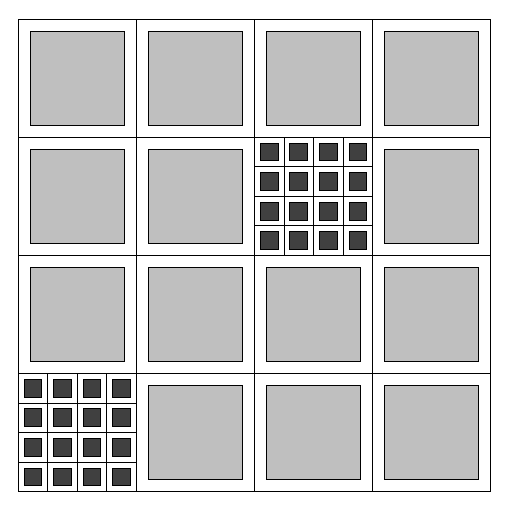
\includegraphics[width=1.8in]{amr4-2.eps} \ \
            \includegraphics[width=1.8in]{amr4-3.eps}}

\centerline{\includegraphics[width=1.8in]{amr4-4.eps} \ \
            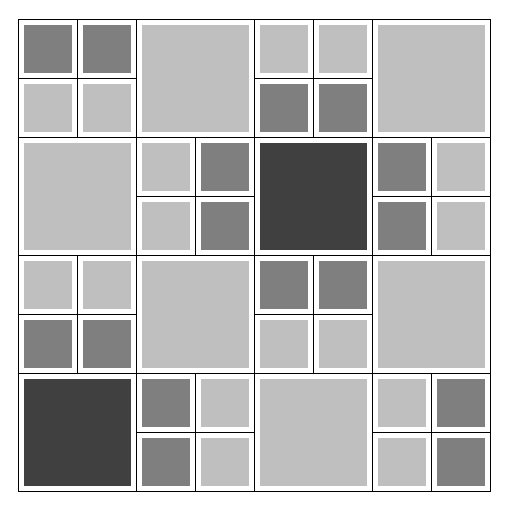
\includegraphics[width=1.8in]{amr4-5.eps} \ \
            \includegraphics[width=1.8in]{amr4-6.eps}}
\centerline{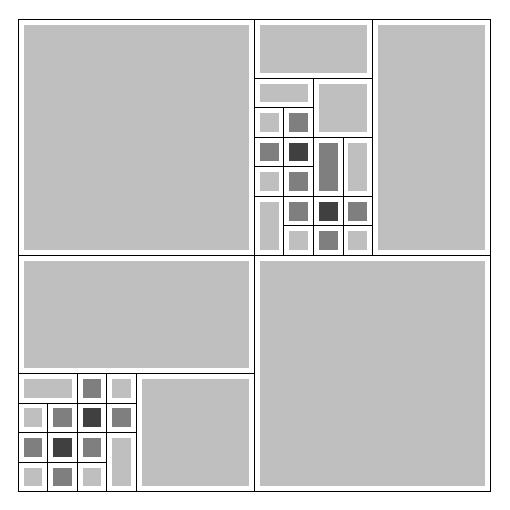
\includegraphics[width=1.8in]{amr4-7.eps}}

% \centerline{\includegraphics[width=1.8in]{amr2-1.eps} \ \
%             \includegraphics[width=1.8in]{amr2-2.eps} \ \
%             \includegraphics[width=1.8in]{amr2-3.eps}}
% \ \\
% \centerline{\includegraphics[width=1.8in]{amr2-4.eps} \ \
%             \includegraphics[width=1.8in]{amr2-5.eps} \ \
%             \includegraphics[width=1.8in]{amr2-7.eps}}
% \ \\
% \centerline{\includegraphics[width=1.8in]{amr2-8.eps} \ \
%             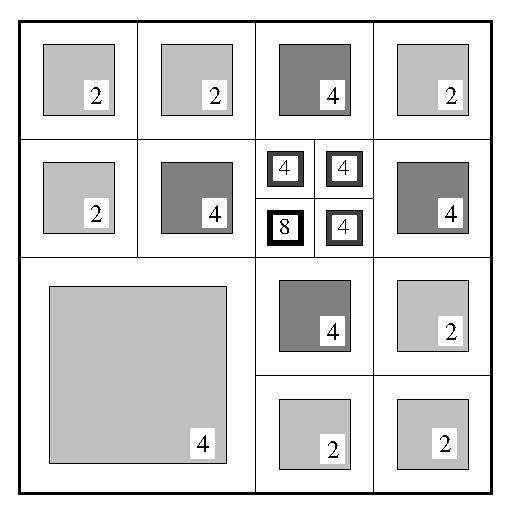
\includegraphics[width=1.8in]{amr2-9.eps} \ \
%             \includegraphics[width=1.8in]{amr2-11.eps}}

%-----------------------------------------------------------------------
\subsection{Use Cases}
%-----------------------------------------------------------------------
%-----------------------------------------------------------------------
\subsection{Parameters}
%-----------------------------------------------------------------------

%=======================================================================
\section{Particle parameters} \label{s:data}
%=======================================================================

Specifies data structures and data structure parameters related
to distributed particles.  

\begin{itemize}
\item min\_group\_size
\item max\_group\_size
\end{itemize}

%-----------------------------------------------------------------------
\subsection{Use Cases}
%-----------------------------------------------------------------------
%-----------------------------------------------------------------------
\subsection{Parameters}
%-----------------------------------------------------------------------

%=======================================================================
\section{Array Component} \label{s:component-array}
%=======================================================================

Use chunked field storage \\
Field chunk size or range
The \code{Array} classes encapsulate Fortran-style arrays with
convenient operations and optional special features.  

Optional features include storing as a blocked array to improve cache
use, array padding to avoid cache thrashing on large power-of-two
arrays with low-associativity caches.  Arrays also may be parallelized
according to \code{Parallel} objects such as
\code{Parallel::Mpi} for MPI-parallel distributed arrays, or
\code{Parallel::Omp} for OpenMP-parallel threaded arrays (or both).

To manage the various optional features, Array classes use the
Decorator design pattern for dynamically adding special features at
run time:

 \centerline{\includegraphics{uml/arrays.ps}}

\subsection{\code{Array}}

\centerline{\includegraphics{uml/array.ps}}

\subsubsection{Array shape}

\subsubsection{Array blocking}

\subsubsection{Array padding}

\subsubsection{Array interleaving}


\subsection{Attributes}

\begin{tabbing}
xx\=xx\=xxxxxxxxxxxxxxxxxxxxxxxxxxxxxxxxxxx\= \kill
\> \todo \>  \textit{Length of array} \\
\>       \> \code{N\_: int }      \\ \\
\> \todo \>  \textit {Shape of array, right-padded with 1's} \\
\>       \> \code{n\_: int [3] }  \\ \\
\> \todo \>  \textit {Array values stored in column-major ordering}\\
\>       \> \code{a\_: Scalar * }
\end{tabbing}

\subsection{Operations}

\begin{tabbing}
xx\=xx\=xxxxxxxxxxxxxxxxxxxxxxxxxxxxxxxxxxx\= \kill
\> \todo \> \textit{Create a new uninitialized Array object} \\
\>       \> \code{Array()} \\ \\
\> \todo \> \textit{Create a new initialized Array object} \\
\>       \> \code{Array(int n0, int n1=1, int n2=1, int n3=1)} \\ \\
\> \todo \> \textit{Deallocate the array} \\
\>       \> \code{\~{\ }Array()}  \\ \\
\> \todo \> \textit{Copy an array into this one, deallocating any existing data} \\
\>       \> \code{void copy (const Array \&)}  \\ \\
\> \todo \> \textit{Resize the array, deallocating any existing data} \\
\>       \> \code{void resize (int n0, int n1=1, int n2=1, int n3=1)}   \\ \\
\> \todo \> \textit{Return the size of the array} \\
\>       \> \code{void size (int *n0, int *n1=0, int *n2=0, int *n3=0) const}  \\ \\
\> \todo \> \textit{Return the total length of the array} \\
\>       \> \code{int length () const}  \\ \\
\> \todo \> \textit{Return a pointer to the array values} \\
\>       \> \code{Scalar * values () const}  \\ \\
\> \todo \> \textit{Return the given array element} \\
\>       \> \code{Scalar \& operator () (int i0, int i1=0, int i2=0, int i3=0)}
\end{tabbing}




%=======================================================================
\section{Parallel Component} \label{s:component-parallel}
%=======================================================================

Hardware platform parallelism will be considered to be multilevel,
including nodes, processors, and cores.  Computational tasks will be
flexibly organized into hierarchical levels to aid mapping to multiple
hardware parallelization levels, including grid patches, grid patch
subblocks, and multiple simulations.  Task sizes in different levels
will allow flexibility to help optimize granularity for the different
given parallelization level components.

Flexible parallelism paradigms: map parallelism to tasks

Automatic code generation (or other) of parallel tasks to implement
parallelism and optimize performance

Specify parallelism type and parameters.  For example, non-blocking
MPI, MPI-2, hybrid MPI/UPC, performance-related parameters such as
buffer size, etc.

Specifiy parallelism and parameters

Specifiy method for controling parallelism

   parallelization method (MPI buffered/blocking, MPI2 Get)

\begin{itemize}
\item MPI (send/recv and type, one-sided and type, what level)
\item OpenMP (num threads, what level)
\item UPC (num threads, what level)
\item pthreads (num threads, what level)
\item cooperative parallelism
\item levels for each if multiple
\end{itemize}

%-----------------------------------------------------------------------
\subsection{Use Cases}
%-----------------------------------------------------------------------
%-----------------------------------------------------------------------
\subsection{Parameters}
%-----------------------------------------------------------------------

%=======================================================================
\subsection{MPI Send/Recv}

%=======================================================================
\subsection{MPI2 Get}

%=======================================================================
\subsection{OpenMP}

%=======================================================================
\subsection{Collaberative parallelism}

%=======================================================================
\subsection{Pipelining}



%=======================================================================
\section{Disk Component} \label{s:component-disk}
%=======================================================================

Output parameters.

%-----------------------------------------------------------------------
\subsection{Use Cases}
%-----------------------------------------------------------------------

\begin{verbatim}
output { 
   name = "data"
   format = hdf5
   type   = [data, input]
   fields = ["density", "velocity", "temperature"]
   file = ["data-%6s" cycle_number]
   cycle = 0:10:90
   cycle = 100:100:900
   cycle = 1000
}
\end{verbatim}

\begin{verbatim}
output { 
   name      = "restart"
   format    = hdf5
   type      = [data, input]
   fields    = all
   file      = ["restart-%6s" cycle_number]
   time_cpu  = 0.5 # CPU hours
   overwrite = true
   copies    = 2
}
\end{verbatim}

\begin{verbatim}
output { 
   name      = "movie"
   file      = ["movie-%6s" cycle_number]
   time      = :10:
   extract   = x == 12
}
\end{verbatim}


%-----------------------------------------------------------------------
\subsection{Parameters}
%-----------------------------------------------------------------------

Output types and parameters
 checkpoint (dump all)
 output (specific fields)
 movies (type and rate)
 analysis (type of analysis, rate)
 level of output (files for timestep, time, etc.)



%=======================================================================
\section{Memory Component} \label{s:component-memory}
%=======================================================================

Dynamic memory allocation.

%-----------------------------------------------------------------------
\subsection{Use Cases}
%-----------------------------------------------------------------------

%-----------------------------------------------------------------------
\subsection{Parameters}
%-----------------------------------------------------------------------





%=======================================================================
\section{Error Component} \label{s:component-error}
%=======================================================================

Fault tolerance and adaptivity parameters

\begin{itemize}
\item fault tolerance methodology
\item adaptivity
\end{itemize}

%-----------------------------------------------------------------------
\subsection{Use Cases}
%-----------------------------------------------------------------------
%-----------------------------------------------------------------------
\subsection{Parameters}
%-----------------------------------------------------------------------

%=======================================================================
\section{Parameters Component} \label{s:component-parameters}
%=======================================================================

The \code{Parameters} component reads in a parameter file or files, and
provides the application access to parameter values.

%-----------------------------------------------------------------------
\subsection{Use Cases}
%-----------------------------------------------------------------------
%-----------------------------------------------------------------------
\subsection{Parameters}
%-----------------------------------------------------------------------



%=======================================================================
\section{Performance Component} \label{s:component-performance}
%=======================================================================
Performance parameters control \lcaperf\ instrumentation.

Performance monitoring and optimization(?) parameters

%-----------------------------------------------------------------------
\subsection{Use Cases}
%-----------------------------------------------------------------------
%-----------------------------------------------------------------------
\subsection{Parameters}
%-----------------------------------------------------------------------

%=======================================================================
\section{Monitor Component} \label{s:component-monitor}
%=======================================================================

High-level monitoring of the run at a summary level, such as current
timestep, problem time, wall time, cpu time, etc.

%-----------------------------------------------------------------------
\subsection{Use Cases}
%-----------------------------------------------------------------------
\begin{verbatim}
   monitor {
     type   = html
     amount = verbose
   }
\end{verbatim}
%-----------------------------------------------------------------------
\subsection{Parameters}
%-----------------------------------------------------------------------

%=======================================================================
\subsection{Performance Component} \label{ss:component-performance}
%=======================================================================
Performance parameters control \lcaperf\ instrumentation.

Performance monitoring and optimization(?) parameters

%-----------------------------------------------------------------------
\subsection{Use Cases}
%-----------------------------------------------------------------------
%-----------------------------------------------------------------------
\subsection{Parameters}
%-----------------------------------------------------------------------


%=======================================================================
\section{Portal Component} \label{s:component-portal}
%=======================================================================


% %=======================================================================
\section{Control parameters} \label{s:control}
%=======================================================================

Given Physics, Algorithms, and Data structures, specify the top-level
sequencing and properties of the simulation.  For example, ordering of
physics modules, whether to do hierarchical time-stepping, up to what
level, whether to sub-cycle some physics, etc. [Is this a useful
category?]  Also include things like floors and limits(?), and IO
dumps

Global simulation control.

Output types and parameters

\begin{itemize}
\item checkpoint (dump all)
\item output (specific fields)
\item movies (type and rate)
\item analysis (type of analysis, rate)
\item level of output (files for timestep, time, etc.)
\end{itemize}

%-----------------------------------------------------------------------
\subsection{Use Cases}
%-----------------------------------------------------------------------
%-----------------------------------------------------------------------
\subsection{Parameters}
%-----------------------------------------------------------------------


% %=======================================================================
\section{Parameters Component} \label{s:component-parameters}
%=======================================================================

The \code{Parameters} component reads in a parameter file or files, and
provides the application access to parameter values.

%-----------------------------------------------------------------------
\subsection{Use Cases}
%-----------------------------------------------------------------------
%-----------------------------------------------------------------------
\subsection{Parameters}
%-----------------------------------------------------------------------


% %=======================================================================
\section{Units parameters} \label{s:units}
%=======================================================================

 Specify units and optional scalings for individual
 fields.  [Merge units with Control?] [Merge scaling with Fields?] 
 [Dynamic scaling, e.g.~to keep average of all fields near one.]

%-----------------------------------------------------------------------
\subsection{Use Cases}
%-----------------------------------------------------------------------
%-----------------------------------------------------------------------
\subsection{Parameters}
%-----------------------------------------------------------------------

% %=======================================================================
\section{Domain Component} \label{s:component-domain}
%=======================================================================

The \code{domain} function is used to specify properties of the
domain.  Domains are boxes aligned with the axes of the computational
coordinate system, and are uniquely determined by the spacial
dimension, and the lowest and highest points in the domain.

%-----------------------------------------------------------------------
\subsection{Use Cases}
%-----------------------------------------------------------------------

\begin{verbatim}
   domain { 
      dimension = 3
      lower     = <-3e9,-3e9,-3e9>
      upper     = <3e9,3e9,3e9>
   }
\end{verbatim}

\begin{verbatim}
   domain { 3, <-3e9,-3e9,-3e9>, <3e9,3e9,3e9> }  // Implicit ordering
\end{verbatim}

\begin{verbatim}
   domain { 
      dimension = 3
      upper     = 3e9        // expand scalar to vector
      lower     = -upper     // parameters can be accessed as values
   }
\end{verbatim}

Include errors.

%-----------------------------------------------------------------------
\subsection{Parameters}
%-----------------------------------------------------------------------

 \todo\ \textit{Decide: allow defaults?  allow optional parameters?  Special
 \code{OPT\_} prefix for optional parameters?  Write out explicit copy
 of input file?}

The \code{domain} function has three parameters

\begin{tabular}{lll} \\
Name & Type & Restrictions \\ \hline
\code{dimension} & Scalar & $1-3$ \\
\code{lower}     & Vector & length = \code{dimension} \\
\code{upper}     & Vector & length = \code{dimension}, \code{upper} $>$ \code{lower}
\end{tabular}

Lower and upper points are given in units given by \code{units},
described in \S\ref{s:units}.

%-----------------------------------------------------------------------
\subsection{Restrictions}
%-----------------------------------------------------------------------

\begin{enumerate}
\item The dimension must be 1, 2, or 3.
\item The number of coordinates in both lower and upper points must equal the dimension.
\item Each coordinate of the lower point must be strictly greater than the corresponding coordinate of the upper point.
\end{enumerate}



% \input{      component-boundary}
% \input{      component-initial}
% 
%=======================================================================
\section{Matter parameters} \label{s:matter}
%=======================================================================

 Matter defines properties of matter, such as the matter type (baryonic
 or dark matter), and gas constants.

%-----------------------------------------------------------------------
\subsection{Use Cases}
%-----------------------------------------------------------------------

\begin{verbatim}
   Matter {
      type = dark
   }
\end{verbatim}

\begin{verbatim}
   Matter {
      type  = gas_ideal
      gamma = 1.4
      region { (x < 0) || (x > 1) }
   }
\end{verbatim}
%-----------------------------------------------------------------------
\subsection{Parameters}
%-----------------------------------------------------------------------

% \input{   component-analysis}
% %=======================================================================
\section{Data Component} \label{s:component-data}
%=======================================================================

Specify low-level datastructures (fields and particles) and their
parameters.

Use chunked field storage \\
Field chunk size or range


%=======================================================================
\subsection{Arrays}

%=======================================================================
\subsection{Fields}

%=======================================================================
\subsection{Particles}

%=======================================================================
\subsection{Structured Adaptive Mesh Hierarchies}

%=======================================================================
\subsection{Octree}


% 
%=======================================================================
\section{Performance Component} \label{s:component-performance}
%=======================================================================
Performance parameters control \lcaperf\ instrumentation.

Performance monitoring and optimization(?) parameters

%-----------------------------------------------------------------------
\subsection{Use Cases}
%-----------------------------------------------------------------------
%-----------------------------------------------------------------------
\subsection{Parameters}
%-----------------------------------------------------------------------


% %------------------------------------------------------------------------
\begin{frame}[fragile] \frametitle{Software Components: High-level}
\end{frame}
%------------------------------------------------------------------------
\begin{frame}[fragile] \frametitle{Control}
      \begin{itemize}
        \item Task: advance grid patch one timestep
        \item Dependencies: boundary values
        \item Dynamic task scheduling
        \begin{itemize}
          \item No artificial dependencies imposed
          \item Patches in different levels can advance concurrently
          \item CHARM++ would be helpful
        \end{itemize}
      \end{itemize}
\end{frame}

% %------------------------------------------------------------------------
\begin{frame}[fragile] \frametitle{Software Components: AMR data structures}
\end{frame}
%------------------------------------------------------------------------
\begin{frame}[fragile] \frametitle{Software Components: \code{Amr}}
\end{frame}

% %------------------------------------------------------------------------
    \begin{frame}[fragile] \frametitle{Software Components: Hardware}
\end{frame}

% %------------------------------------------------------------------------
    \begin{frame}[fragile] \frametitle{Software Components: AMR data structures}
\end{frame}

% \include{components-support}

%========================================================================
\section{Data structures}
%========================================================================

%------------------------------------------------------------------------
\subsection{Related applications}
%------------------------------------------------------------------------

%------------------------------------------------------------------------
\begin{frame}[fragile] \frametitle{Chombo: Patch-based AMR}
\begin{minipage}{1.5in}
\centerline{\includegraphics[width=1.5in]{chombo.png}}
\end{minipage} \ 
\begin{minipage}{2.5in}
\begin{itemize}
\enhance{1}\item Colella et al, LBNL
\enhance{2}\item Patch-based with overlayed octree
\enhance{3}\item Parallel grid refinement algorithm
\enhance{4}\item Patches may have multiple parents
\enhance{5}\item Patches are properly nested
\end{itemize}
\end{minipage}
\end{frame}

%------------------------------------------------------------------------
\begin{frame}[fragile] \frametitle{FLASH / Paramesh: Tree-based AMR}
\centerline{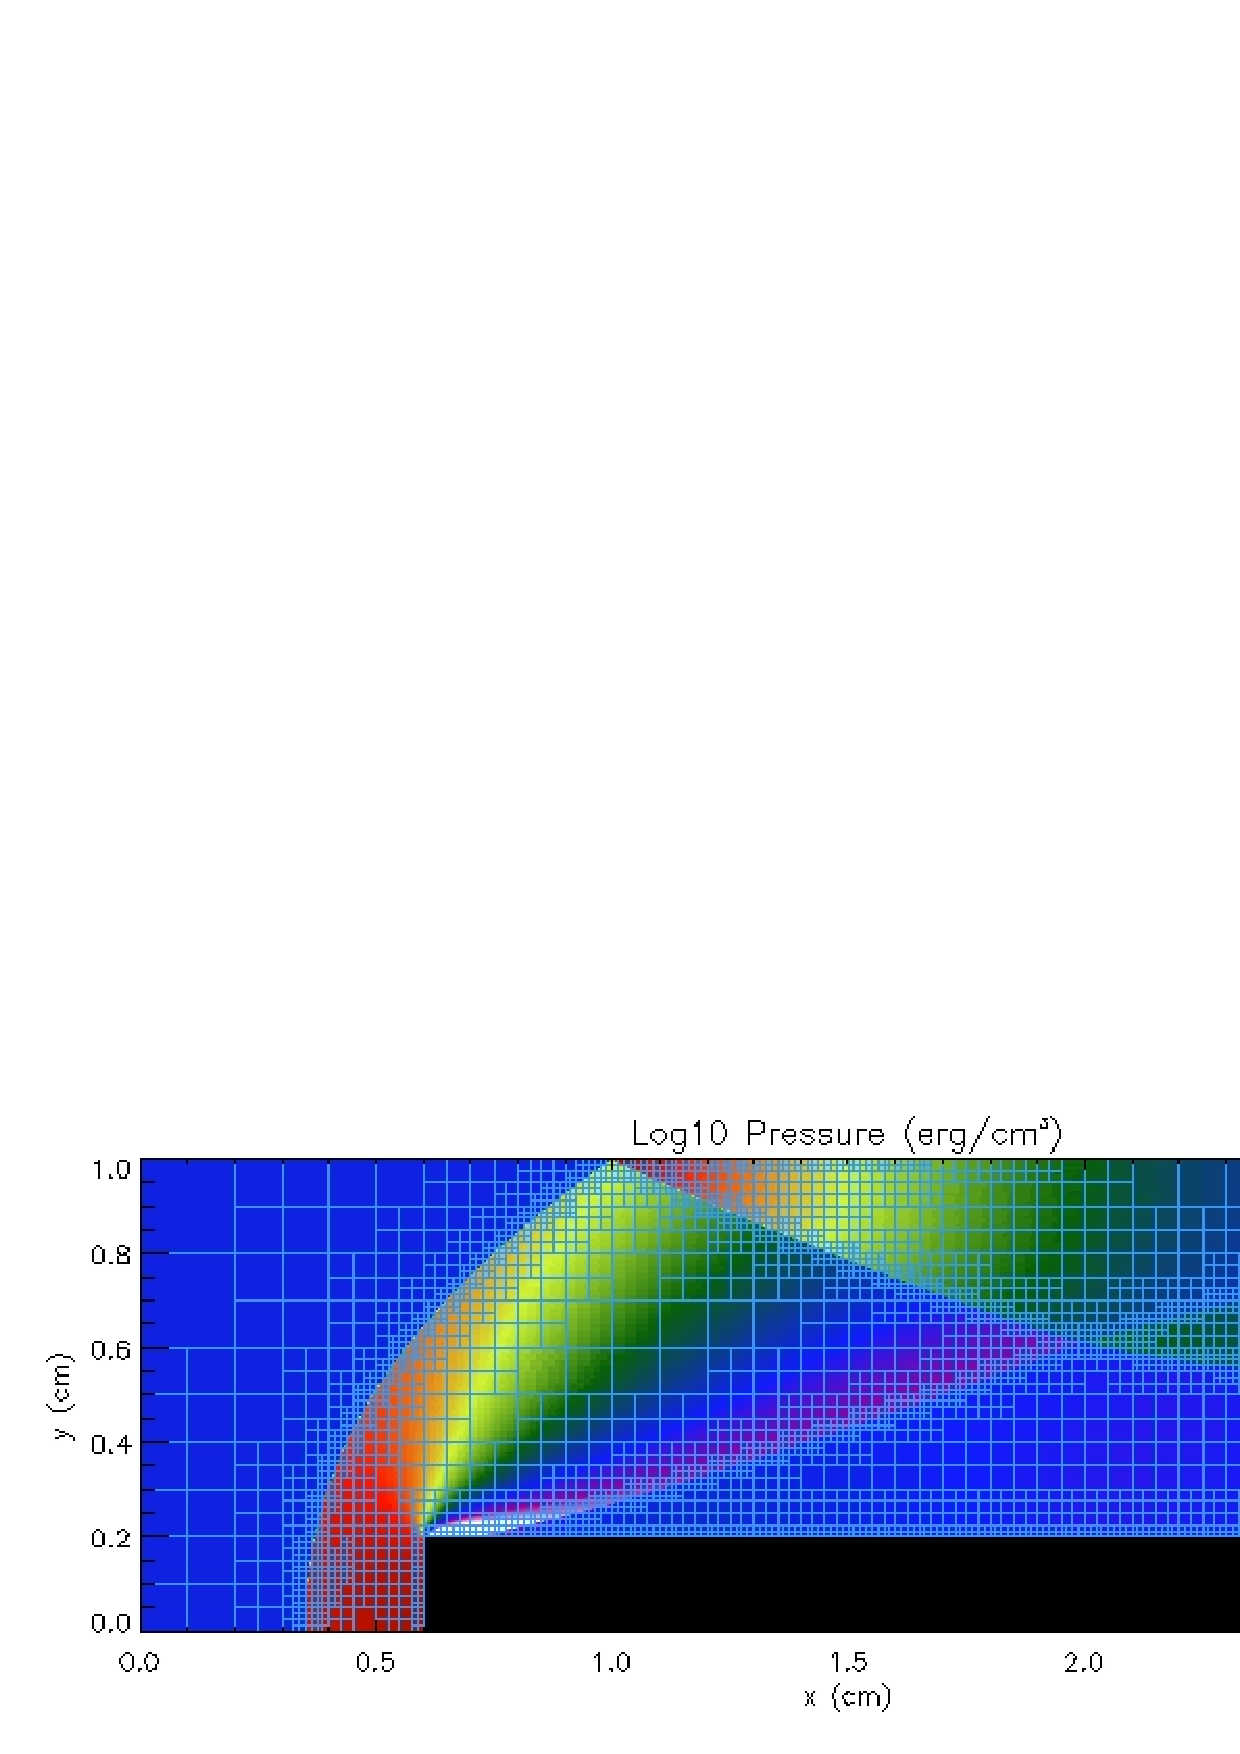
\includegraphics[width=3.0in]{paramesh.png}}
\begin{minipage}{2.3in}
\begin{itemize}
\enhance{1}\item ASCI/Alliance FLASH Center
\enhance{2}\item $>500,000$ lines of code
\enhance{3}\item Uniform time-stepping
\end{itemize}
\end{minipage}
\begin{minipage}{1.8in}
\begin{itemize}
\enhance{4}\item $2^d$-tree refinement 
\enhance{5}\item Fixed sized patches
\enhance{6}\item No ``level-jumps''
\end{itemize}
\end{minipage}

\end{frame}

% \end{minipage} \
% \begin{minipage}{2in}
% \begin{itemize}
% \enhance{2}\item[+] Easier grid generation
% \enhance{3}\item[+] Fast neighbor search
% \enhance{4}\item[+] Easier to load balance
% \enhance{5}\item[+] Regularly-sized grids
% \end{itemize}
% \end{minipage} \
% \begin{minipage}{2in}
% \begin{itemize}
% \enhance{6}\item[-] More grid patches
% \enhance{7}\item[-] Small grid patches
% \end{itemize}
% \end{minipage}
% 
% \end{frame}

%------------------------------------------------------------------------
\begin{frame}[fragile] \frametitle{\cello: Hybrid Patch-AMR and Tree-AMR}

\begin{minipage}{2in}
\begin{itemize}
\enhance{1}\item Patch-based AMR ala Chombo
\enhance{2}\item Modified tree-based AMR ala FLASH
\begin{itemize}
\enhance{3}\item Patch-reduction
\enhance{4}\item $k^d$-d refinement
\end{itemize}
\enhance{5}\item Much code reuse between patch- and tree-AMR
\end{itemize}
\end{minipage}
\begin{minipage}{2.0in}
\centerline{\includegraphics[width=2.0in]{norman.png}}
\end{minipage}
\end{frame}

%------------------------------------------------------------------------
    \begin{frame}[fragile] \frametitle{Review of AMR Applications}
    \footnotesize
      \begin{tabular}{|l|ccc|cc|}
\hline
    &  \textbf{Enzo} & \textbf{Chombo} & \textbf{FLASH} & \textbf{Cello-patch} & \textbf{Cello-tree} \\  \hline
    \textbf{Refinement} &  \enhanceus{2}{patch} & \enhancethem{3}{patch} &  \enhancethem{4}{$2^d$-tree} & \enhancenewus{5}{patch} & \enhancenewus{6}{$k^d$-tree}  \\
%    \textbf{Tree type} & \enhanceus{2}{none} & \enhancethem{3}{octree} & \enhancethem{4}{octree} & \enhancenewus{5}{octree} & \enhancenewus{6}{octree++} \\  \hline
    \textbf{Patch shape} & \enhanceus{2}{  variable} & \enhancethem{3}{variable} &  \enhancethem{4}{constant} & \enhancenewus{5}{variable} & \enhancenewus{6}{constant} \\
    \textbf{Patch size} & \enhanceus{2}{  variable} & \enhancethem{3}{variable} &  \enhancethem{4}{constant} & \enhancenewus{5}{variable} &\enhancenewus{6}{limited}  \\ \hline
    \textbf{Parents} & \enhanceus{2}{single} & \enhancethem{3}{multiple} & \enhancethem{4}{single} &   \enhancenewus{5}{multiple} & \enhancenewus{6}{single} \\
    \textbf{Children} & \enhanceus{2}{variable} & \enhancethem{3}{variable} & \enhancethem{4}{constant} & \enhancenewus{5}{variable} & \enhancenewus{6}{limited} \\
    \textbf{Neighbors} & \enhanceus{2}{variable} & \enhancethem{3}{variable} & \enhancethem{4}{limited} & \enhancenewus{5}{variable} & \enhancenewus{6}{limited} \\\hline
    \textbf{Level jumps} & \enhanceus{2}{ yes} &    \enhancethem{3}{no} &      \enhancethem{4}{no}    &   \enhancenewus{5}{no} & \enhancenewus{6}{no} \\
    \textbf{Asymmetric} & \enhanceus{2}{yes} &  \enhancethem{3}{no} &  \enhancethem{4}{no} &  \enhancenewus{5}{no} & \enhancenewus{6}{no} \\\hline
      \end{tabular}
\end{frame}


%------------------------------------------------------------------------
\subsection{AMR versus unigrid}
%------------------------------------------------------------------------

%------------------------------------------------------------------------
\begin{frame}[fragile] \frametitle{\cello\ AMR philosophy}
\begin{itemize}
\enhance{1}\item \code{Array}s are preferred for uniform resolution regions
\enhance{2}\item \code{Amr} data structures required for multi-resolution
\enhance{3}\item Issues with standard tree-based AMR
\begin{itemize}
\enhance{4}\item Lots of small patches at finest resolution
\enhance{5}\item $2^d$-tree refinement is too ``shallow'' for deep AMR
\end{itemize}
\enhance{6}\item Three proposed modifications:
\begin{itemize}
\enhance{7}\item Patch coalescing
\enhance{8}\item Individual child refinement
\enhance{9}\item $k^d$ refinement with backfill
\end{itemize}
\end{itemize}
\end{frame}




%----------------------------------------------------------------------
\begin{frame}
\frametitle{Cello Arrays}
\begin{minipage}{2.0in}
\begin{itemize}
\enhance{1}\item Generalized Fortran array
\enhance{2}\item MPI-[12], OMP, UPC
\enhance{3}\item Blocking / padding
\end{itemize}
\end{minipage} \ 
\begin{minipage}{2.0in}
\begin{itemize}
\enhance{4}\item C++ / Fortran interface
\enhance{5}\item Iterators over blocks
\enhance{6}\item Unigrid is single \code{Array}
\end{itemize}
\end{minipage}
\begin{minipage}{1.3in}
\vspace{0.1in}
\begin{itemize}
\item[]\includegraphics[width=0.4in]{array-serial.png} \ \ \code{ArraySerial}
\item[]\includegraphics[width=0.4in]{array-block.png} \ \ \code{ArrayBlock}
\end{itemize}
\end{minipage} \ 
\begin{minipage}{1.3in}
\vspace{0.1in}
\begin{itemize}
\item[]\includegraphics[width=0.4in]{array-mpi.png} \ \ \code{ArrayMpi}
\item[]\includegraphics[width=0.4in]{array-omp.png} \ \ \code{ArrayOmp}
\end{itemize}
\end{minipage} \ 
\begin{minipage}{1.3in}
\vspace{0.1in}
\begin{itemize}
\item[]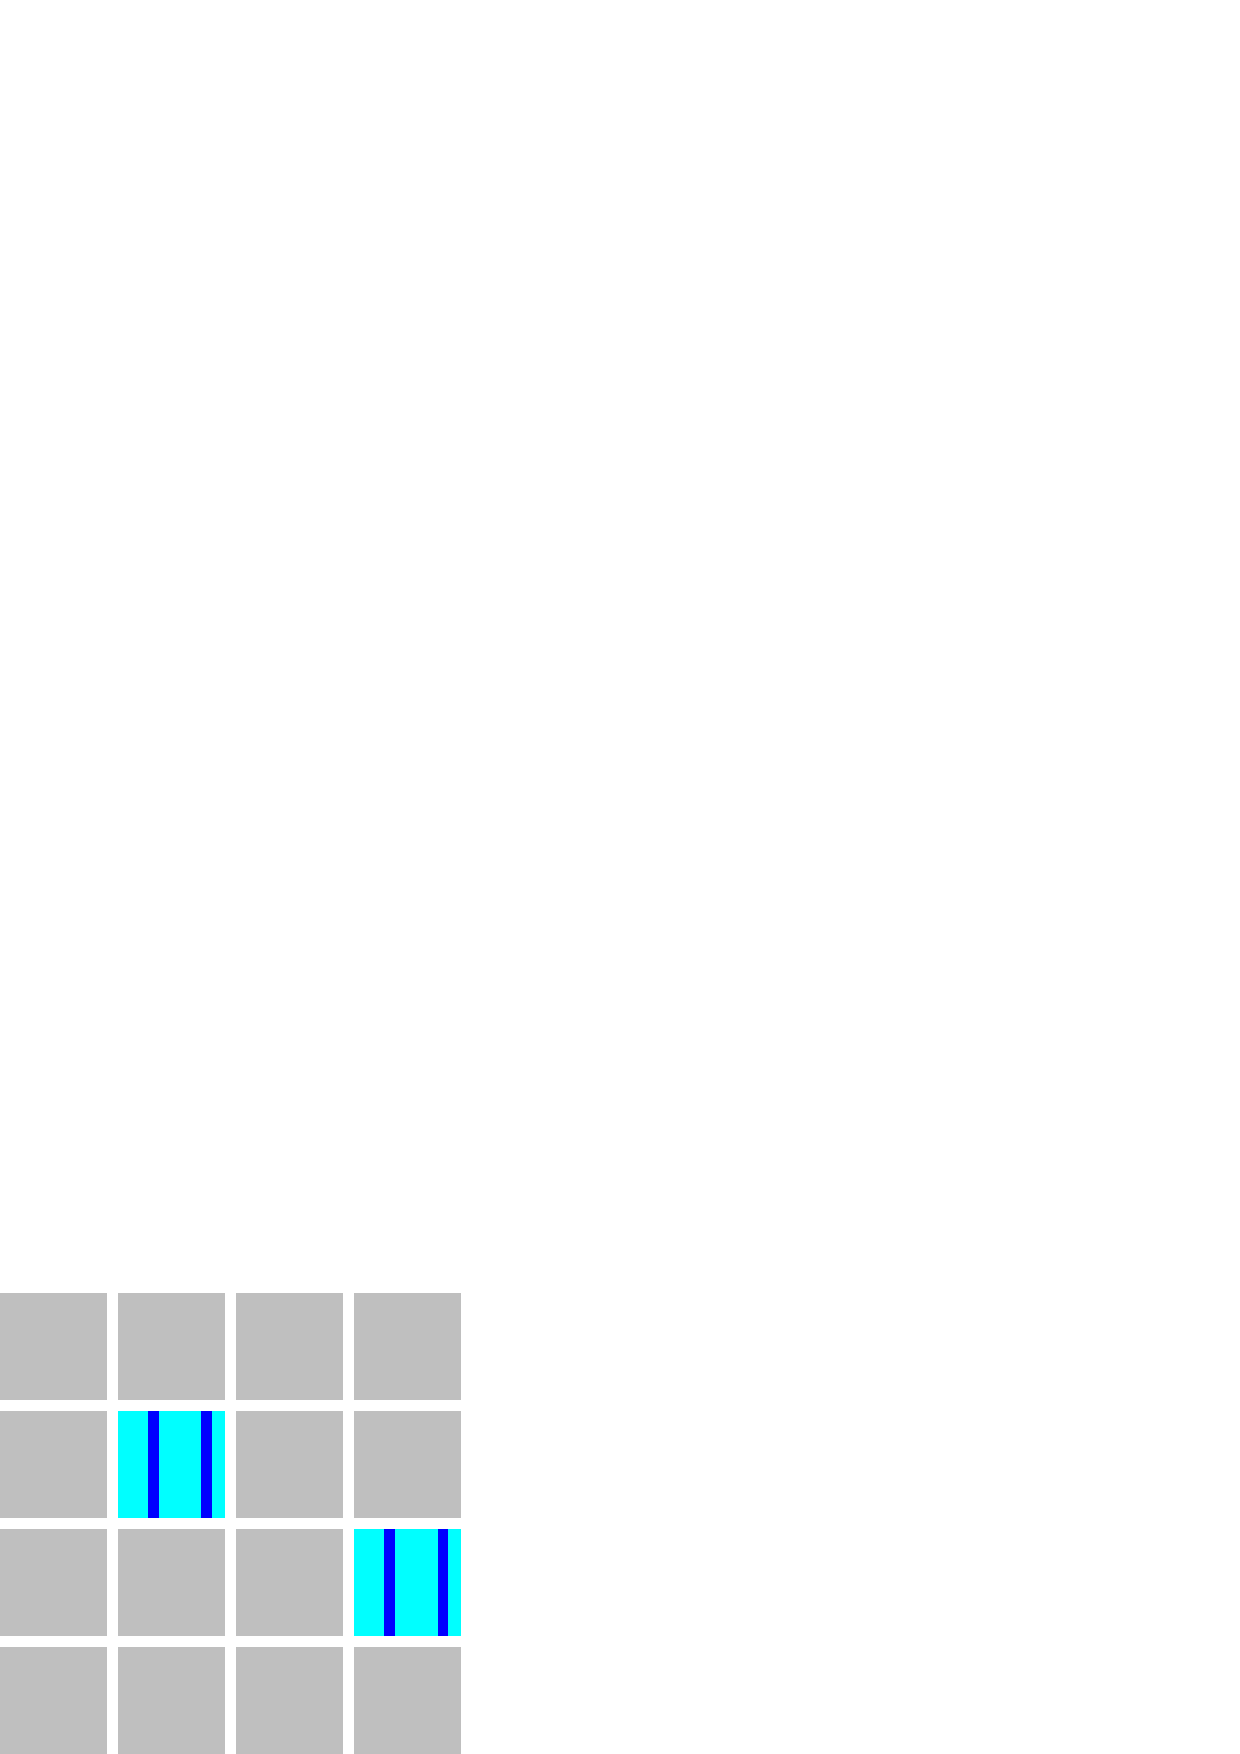
\includegraphics[width=0.4in]{array-mpi-omp.png} \ \ \code{ArrayMpiOmp}
\item[]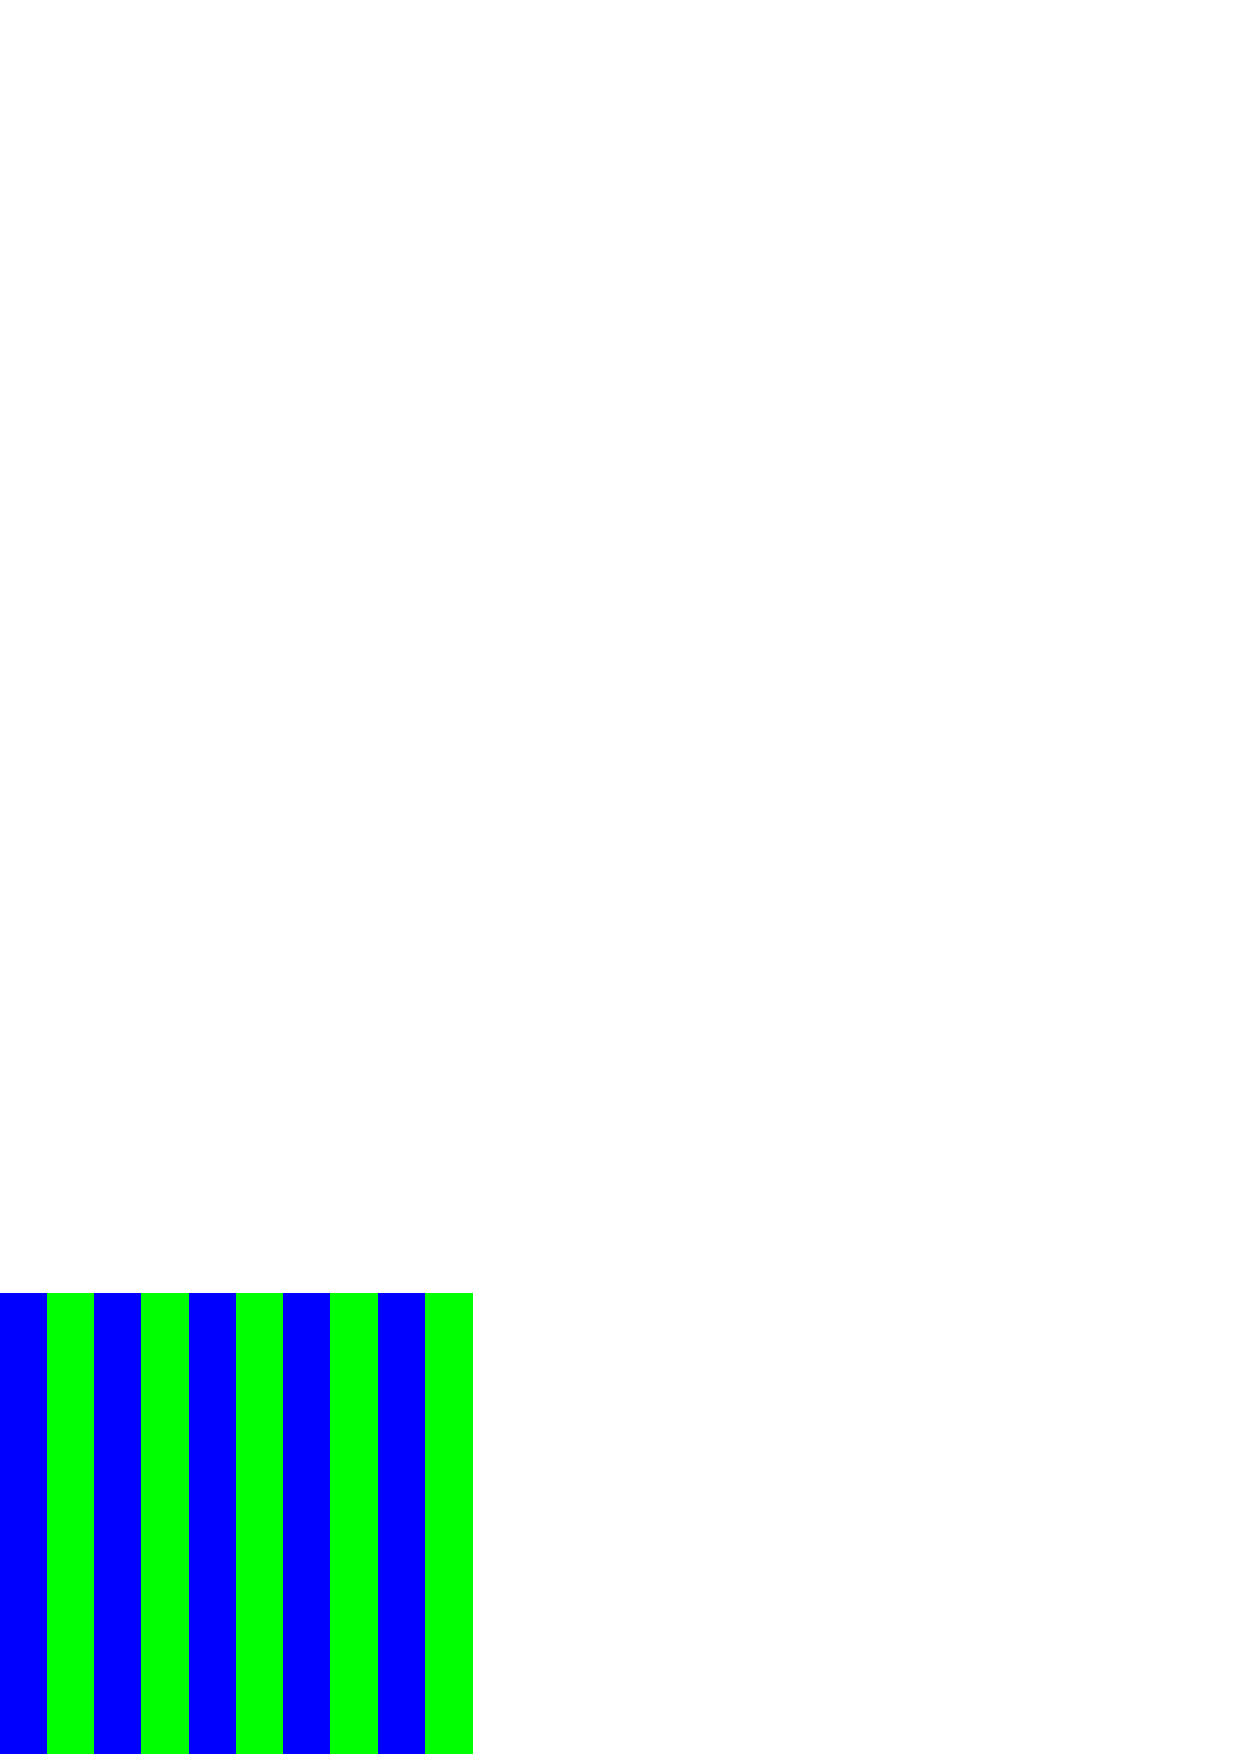
\includegraphics[width=0.4in]{array-interleave.png} \ \ \code{ArrayInterleave}
\end{itemize}
\end{minipage}

\end{frame}
%----------------------------------------------------------------------

\begin{frame}[fragile] \frametitle{Cello AMR: Patch Coalescing}
\centerline{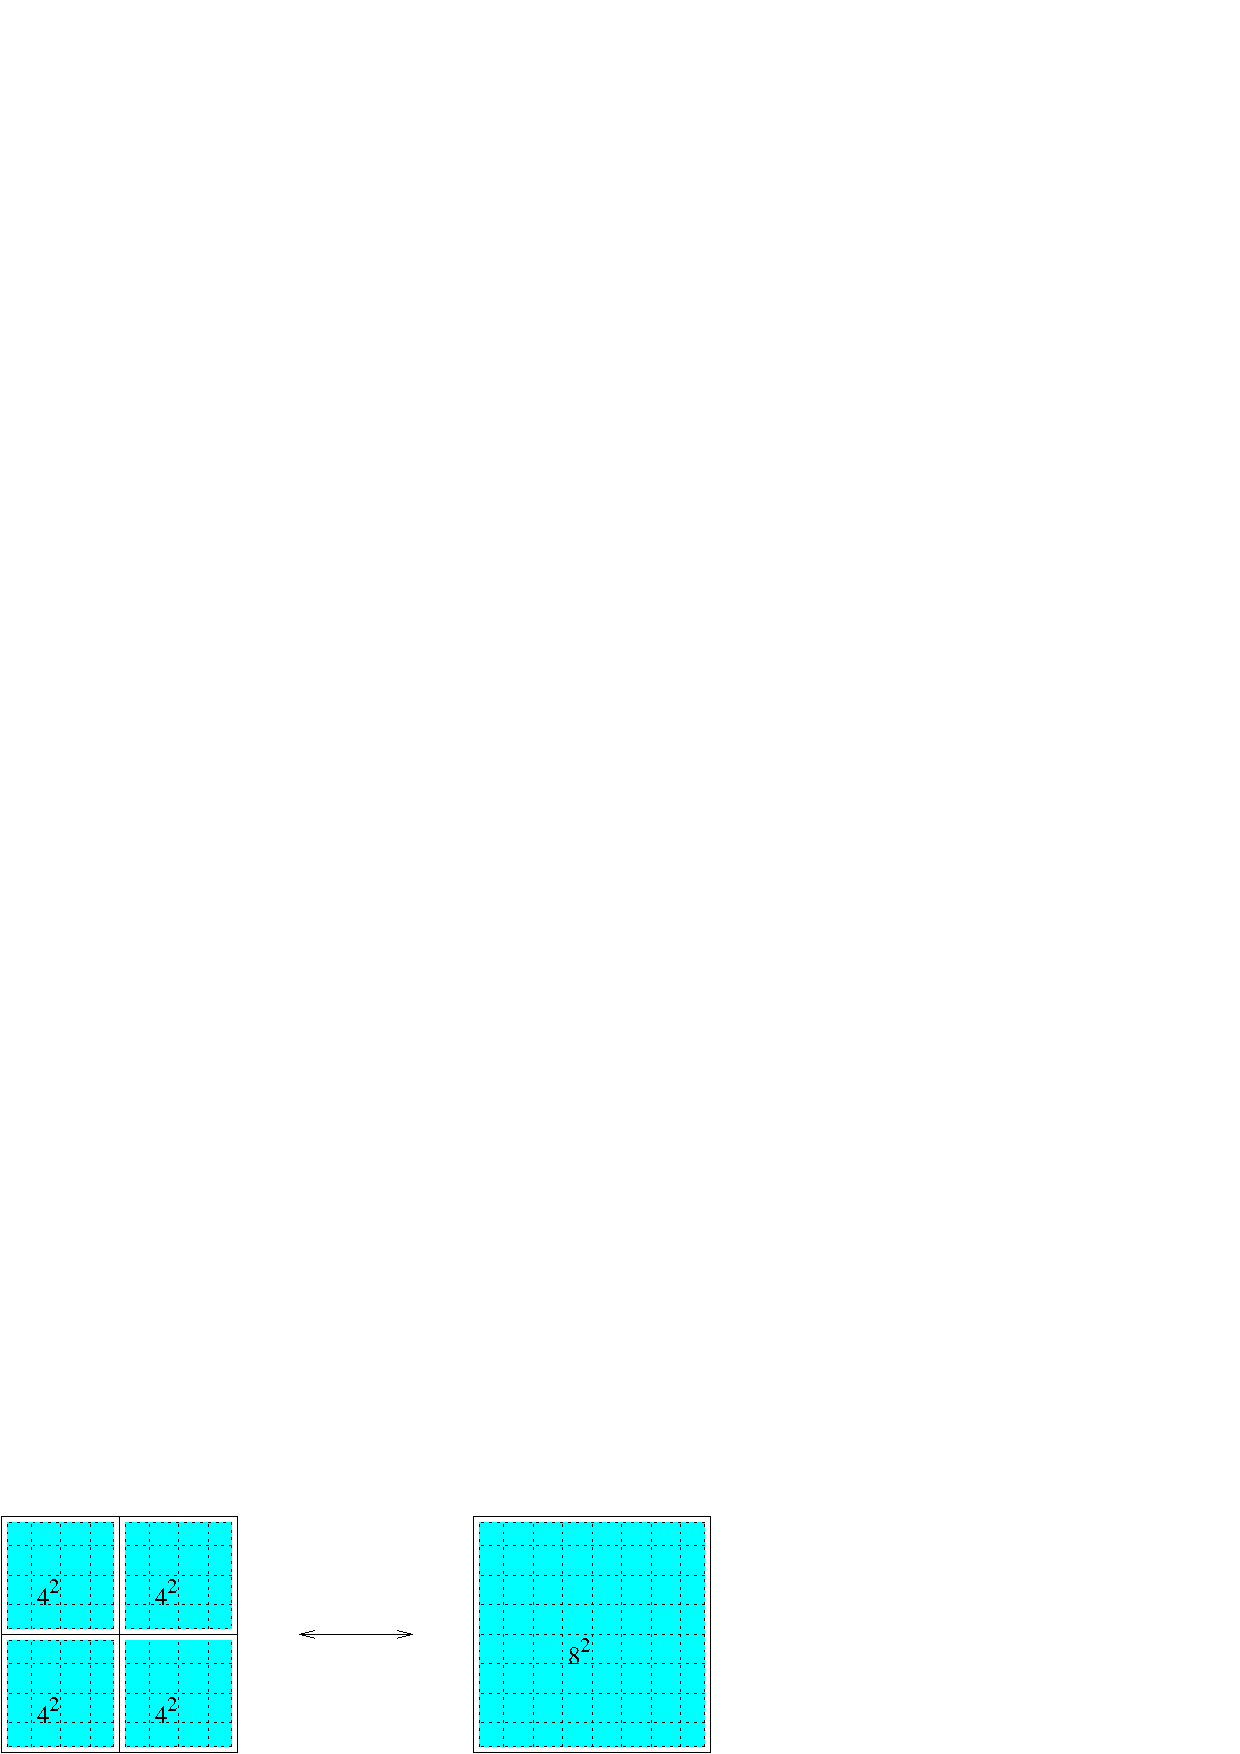
\includegraphics[width=2.5in]{coalesce.png}}
\begin{itemize}
\enhance{2}\item Replace AMR nodes with larger arrays when possible
\enhance{3}\item Replace arrays with AMR nodes when necessary
\enhance{4}\item Allows adapting to constant versus changing resolution
\end{itemize}
\end{frame}

\begin{frame}[fragile] \frametitle{Cello AMR: Individual Child Refinement}
\centerline{\includegraphics[width=2.5in]{amr-child.png}}
\begin{itemize}
\enhance{1}\item Refine children individually instead of all or nothing
\enhance{2}\item Added flexibility can reduce AMR tree size
\end{itemize}
\end{frame}

\begin{frame}[fragile] \frametitle{Cello AMR: $k^d$ Refinement with Backfill}
\centerline{\includegraphics[width=3.5in]{kd-backfill.png}}
\begin{itemize}
\enhance{1}\item If $k=4$, refine by $4$ instead of $2$
\enhance{2}\item More ``targeted'' refinement
\enhance{3}\item Can optionally remove level jumps by ``backfilling'' levels
\enhance{4}\item Backfill patch locations are known implicitly---nominal storage
\enhance{5}\item Many child nodes implies sparse storage
\end{itemize}
\end{frame}


%------------------------------------------------------------------------
\subsection{Tree-AMR examples}
%------------------------------------------------------------------------

%------------------------------------------------------------------------
    \begin{frame}[fragile] \frametitle{Point-source test: $2^d$-trees}
\begin{minipage}{2.3in}
\includegraphics<1>[width=2.3in]{dots.png}
\includegraphics<2>[width=2.3in]{dots-4-0.png}
\includegraphics<3>[width=2.3in]{dots-4-1.png}
\includegraphics<4>[width=2.3in]{dots-4-2.png}
\end{minipage}
\begin{minipage}{1.6in}
\footnotesize
      \begin{itemize}
        \item \ENHANCE{1}Test problem: refine on point sources
        \item \ENHANCE{2}Simple quad-tree has level jumps
        \item \ENHANCE{3}Normalization helps, but issues remain
        \begin{itemize}
\footnotesize
          \item \ENHANCE{3}numerous patches
          \item \ENHANCE{3}slow refinement
        \end{itemize}
        \item \ENHANCE{4}Patch coalescing reduces patch count
      \end{itemize}
\end{minipage} \\
\begin{minipage}{4.0in}
\footnotesize
Nodes: 
\ENHANCE{2}549
\ENHANCE{3}2137
\ENHANCE{4}\textbf{1073}
\color{lightgray}155
\color{lightgray}650
\color{lightgray}\textbf{650}
\color{lightgray}86
\color{lightgray}158
\color{lightgray}\textbf{158}
\end{minipage}
\end{frame}

%------------------------------------------------------------------------
    \begin{frame}[fragile] \frametitle{Point-source test: child-refinement}
\begin{minipage}{2.3in}
\includegraphics<1>[width=2.3in]{dots-4-3.png}
\includegraphics<2>[width=2.3in]{dots-4-4.png}
\includegraphics<3>[width=2.3in]{dots-4-5.png}
\end{minipage} \
\begin{minipage}{1.6in}
\footnotesize
      \begin{itemize}
        \item \ENHANCE{1}Try refining subset of children
        \item \ENHANCE{2}Still have to deal with level jumps
        \item \ENHANCE{3}Patch coalescing not effective
      \end{itemize}
\end{minipage} \\
\begin{minipage}{4.0in}
\footnotesize
Nodes: 
\color{gray}549
\color{gray}2137
\color{gray}\textbf{1073}
\ENHANCE{1}155
\ENHANCE{2}650
\ENHANCE{3}\textbf{650}
\color{lightgray}86
\color{lightgray}158
\color{lightgray}\textbf{158}

\end{minipage}
\end{frame}

%------------------------------------------------------------------------

    \begin{frame}[fragile] \frametitle{Point-source test: $4^d$-trees + child-refinement}
\begin{minipage}{2.3in}
\includegraphics<1>[width=2.3in]{dots-16-3.png}
\includegraphics<2>[width=2.3in]{dots-16-4.png}
\includegraphics<3>[width=2.3in]{dots-16-5.png}
\includegraphics<4>[width=2.3in]{dots-16-5.png}
\end{minipage} \
\begin{minipage}{1.6in}
\footnotesize
      \begin{itemize}
        \item \ENHANCE{1}Try refinement by 4 instead of 2
        \item \ENHANCE{2}Deal with level jumps
        \item \ENHANCE{3}Patch coalescing still not effective
        \item \ENHANCE{4}Still relatively good
      \begin{itemize}
\footnotesize
        \item \ENHANCE{4}Fewer patches
	\item \ENHANCE{4}Steep refinement
        \item \ENHANCE{4}Can 'back-fill' to regain refinement-by-2
      \end{itemize}
      \end{itemize}
\end{minipage}
\begin{minipage}{4.0in}
\footnotesize
Nodes: 
\color{gray}549
\color{gray}2137
\color{gray}\textbf{1073}
\color{gray}155
\color{gray}650
\color{gray}\textbf{650}
\ENHANCE{1}86
\ENHANCE{2}158
\ENHANCE{3-4}\textbf{158}

\end{minipage}
\end{frame}

%------------------------------------------------------------------------

    \begin{frame}[fragile] \frametitle{Cosmology Test: $2^d$-Trees}
\begin{minipage}{4.0in}
\footnotesize
Nodes:
\ENHANCE{2}61261
\ENHANCE{3}81701
\ENHANCE{4}\textbf{32529}
\color{lightgray}35608
\color{lightgray}43950
\color{lightgray}\textbf{35942}
\color{lightgray}33542
\color{lightgray}33868
\color{lightgray}\textbf{31708} \\
\end{minipage} 
\begin{minipage}{2.2in}
\includegraphics<1>[width=2.2in]{cosmo2.png}
\includegraphics<2>[width=2.2in]{cosmo2-4-0.png}
\includegraphics<3>[width=2.2in]{cosmo2-4-1.png}
\includegraphics<4>[width=2.2in]{cosmo2-4-2.png}
\end{minipage} \
\begin{minipage}{1.6in}
\footnotesize
      \begin{itemize}
        \item \ENHANCE{1}Test problem: 2D cosmology image
        \item \ENHANCE{2}Basic $2^d$ tree
        \item \ENHANCE{3}Normalize for level jumps
        \item \ENHANCE{4}Coalesce patches
      \end{itemize}
\end{minipage}
\end{frame}

%------------------------------------------------------------------------

    \begin{frame}[fragile] \frametitle{Cosmology Test: $2^k$-Trees with Child-Refinement}
\begin{minipage}{4.0in}
\footnotesize
Nodes:
\color{gray}61261
\color{gray}81701
\color{gray}\textbf{32529}
\ENHANCE{1}35608
\ENHANCE{2}43950
\ENHANCE{3}\textbf{35942}
\color{lightgray}33542
\color{lightgray}33868
\color{lightgray}\textbf{31708} \\
\end{minipage}
\begin{minipage}{2.2in}
\includegraphics<1>[width=2.2in]{cosmo2-4-3.png}
\includegraphics<2>[width=2.2in]{cosmo2-4-4.png}
\includegraphics<3>[width=2.2in]{cosmo2-4-5.png}
\end{minipage} \
\begin{minipage}{1.6in}
\footnotesize
      \begin{itemize}
        \item \ENHANCE{1}Refine on subset of children
        \item \ENHANCE{2}Normalize for level jumps
        \item \ENHANCE{3}Coalesce patches
      \end{itemize}
\end{minipage}
\end{frame}
%------------------------------------------------------------------------

    \begin{frame}[fragile] \frametitle{Cosmology Test: $4^d$-Trees with Child-Refinement}
\begin{minipage}{4.0in}
\footnotesize
Nodes:
\color{gray}61261
\color{gray}81701
\color{gray}\textbf{32529}
\color{gray}35608
\color{gray}43950
\color{gray}\textbf{35942}
\ENHANCE{1}33542
\ENHANCE{2}33868
\ENHANCE{3}\textbf{31708} \\
\end{minipage}
\begin{minipage}{2.2in}
\includegraphics<1>[width=2.2in]{cosmo2-16-3.png}
\includegraphics<2>[width=2.2in]{cosmo2-16-4.png}
\includegraphics<3>[width=2.2in]{cosmo2-16-5.png}
\end{minipage} \
\begin{minipage}{1.6in}
\footnotesize
      \begin{itemize}
        \item \ENHANCE{1}$4^d$-tree refinement
        \item \ENHANCE{2}Normalize for level jumps
        \item \ENHANCE{3}Coalesce patches
      \end{itemize}
\end{minipage}
\end{frame}


%========================================================================
\section{Issues and solutions}
%========================================================================

%------------------------------------------------------------------------
    \begin{frame}[fragile] \frametitle{Concurrent level time-stepping}
\begin{minipage}{1.3in}
\includegraphics<1->[width=1.3in]{timestep-levels.png}
\end{minipage} \
\begin{minipage}{1.3in}
\includegraphics<2->[width=1.3in]{timestep-dynamic.png}
\end{minipage} \
\begin{minipage}{1.3in}
\includegraphics<5->[width=1.3in]{timestep-uniform.png}
\end{minipage} \
\begin{itemize}
\enhance{1}\item \enzo\ time-stepping proceeds level by level
\enhance{2}\item Levels may proceed concurrently
  \begin{itemize}
  \enhance{3}\item[$+$] Faster if enough parallelism
  \enhance{4}\item[$-$] Reduced parallel efficiency
  \end{itemize}
\enhance{5}\item Uniform time-stepping possible option
  \begin{itemize}
  \enhance{6}\item[$+$] Improved parallel efficiency
  \enhance{6}\item[$+$] Faster if enough parallelism
  \enhance{7}\item[$-$] More overall work
  \end{itemize}
\end{itemize}
\end{frame}

%------------------------------------------------------------------------
\begin{frame}[fragile] \frametitle{Particle positions}
\vspace{-0.2in}
\begin{minipage}{1.8in}
\includegraphics<1->[width=2.0in]{particles-global.png}
\end{minipage} \
\begin{minipage}{2.0in}
\includegraphics<3->[width=2.0in]{particles-local.png}
\end{minipage} \
      \begin{itemize}
        \enhance{1}\item Precision issues with deep AMR
        \enhance{2}\item Patch-local coordinates could address this
        \enhance{3}\item Coordinate changes still accurate
        \enhance{4}\item Single-precision may be sufficient (exponent?)
      \end{itemize}
\end{frame}

%------------------------------------------------------------------------
    \begin{frame}[fragile] \frametitle{Hierarchical Load balancing}
\end{frame}

%------------------------------------------------------------------------
    \begin{frame}[fragile] \frametitle{Precision issues: Grids}
      \begin{itemize}
        \item Define grid location only relative to neighboring grid
        \item 32-bit integers always sufficient
        \item No global tree structure
        \item Issues
        \begin{itemize}
          \item Load balancing
          \begin{itemize}
            \item CHARM++
          \end{itemize}
          \item Re-gridding
          \begin{itemize}
            \item local algorithm
          \end{itemize}
          \item Global time step
        \end{itemize}
        \item High scalability
      \end{itemize}
\end{frame}

%------------------------------------------------------------------------
    \begin{frame}[fragile] \frametitle{Gravity}
      \begin{itemize}
        \item Hypre insufficient
        \begin{itemize}
          \item Best method FAC is unusable
        \end{itemize}
        \item Write own FAC
        \item Chombo group is on top of this
      \end{itemize}
\end{frame}

%------------------------------------------------------------------------
\begin{frame}[fragile] \frametitle{Software Resiliency}
\begin{itemize}
\enhance{1}  \item Handle software / hardware errors gracefully
  \begin{itemize}
\enhance{2}     \item Identify problems: memory error, node crash, etc.
\enhance{3}     \item Bactrack and continue on reduced hardware
  \end{itemize}
\enhance{4}  \item Use checkpoint/restart library, e.g.~BLCR
\enhance{5}  \item Application / library determines best checkpoint frequency
\enhance{6}  \item Minimize size of checkpoint dumps
  \end{itemize}
\end{frame}


%========================================================================
\section{Conclusions}
%========================================================================

%%%%%%%%% MASTER -- compiles the 4 sections

\documentclass[11pt,letterpaper]{article}

%%%%%%%%%%%%%%%%%%%%%%%%%%%%%%%%%%%%%%%%%%%%%%%%%%%%%%%%%%%%%%%%%%%%%%%%%
\pagestyle{plain}                                                      %%
%%%%%%%%%% EXACT 1in MARGINS %%%%%%%                                   %%
\setlength{\textwidth}{6.5in}     %%                                   %%
\setlength{\oddsidemargin}{0in}   %% (It is recommended that you       %%
\setlength{\evensidemargin}{0in}  %%  not change these parameters,     %%
\setlength{\textheight}{8.5in}    %%  at the risk of having your       %%
\setlength{\topmargin}{0in}       %%  proposal dismissed on the basis  %%
\setlength{\headheight}{0in}      %%  of incorrect formatting!!!)      %%
\setlength{\headsep}{0in}         %%                                   %%
\setlength{\footskip}{.5in}       %%                                   %%
%%%%%%%%%%%%%%%%%%%%%%%%%%%%%%%%%%%%                                   %%
\newcommand{\required}[1]{\section*{\hfil #1\hfil}}                    %%
\renewcommand{\refname}{\hfil References Cited\hfil}                   %%
\bibliographystyle{plain}                                              %%
%%%%%%%%%%%%%%%%%%%%%%%%%%%%%%%%%%%%%%%%%%%%%%%%%%%%%%%%%%%%%%%

\usepackage{epsfig}
\usepackage{url}

\newcommand{\cello}{\textsf{Cello}}
\newcommand{\enzo}{\textsf{Enzo}}
\newcommand{\enzoii}{\textsf{Enzo}-\texttt{II}}
\newcommand{\lcaperf}{\textsf{lcaperf}}
\newcommand{\lcatest}{\textsf{lcatest}}

\newcommand{\pp}{\texttt{++}}
\newcommand{\cpp}{C\pp}
\newcommand{\charm}{\textsf{Charm\pp}}
\newcommand{\chombo}{\textsf{Chombo}}
\newcommand{\samrai}{\textsf{SAMRAI}}
\newcommand{\paramesh}{\textsf{PARAMESH}}
\newcommand{\gadget}{\textsf{GADGET}}
\newcommand{\alps}{\textsf{ALPS}}
\newcommand{\clawpack}{\textsf{CLAWPACK}}
\newcommand{\grace}{\textsf{GrACe}}
\newcommand{\carpet}{\textsf{Carpet}}
\newcommand{\flash}{\textsf{FLASH}}

\newcommand{\code}[1]{\textsf{#1}}

\newcounter{figctr}

\newcommand{\FIGURE}[3]{
\noindent
\parbox{\textwidth}{
%\ \\ \hrule \ \\
\begin{center}
#3
\end{center}%
\ \nolinebreak%
\refstepcounter{figctr}%
\begin{center}%
\begin{minipage}{7.0in}
\textbf{Figure \thefigctr}. #1
\end{minipage}
\end{center}
\label{#2}
%\ \\ \hrule \ \\
}}

% NSF proposal generation template style file.
% based on latex stylefiles  written by Stefan Llewellyn Smith and
% Sarah Gille, with contributions from other collaborators.

\DeclareFontFamily{OT1}{psyr}{}
\DeclareFontShape{OT1}{psyr}{m}{n}{<-> psyr}{}
\def\times{{\fontfamily{psyr}\selectfont\char180}}


\renewcommand{\refname}{\centerline{References cited}}

% this handles hanging indents for publications
\def\rrr#1\\{\par
\medskip\hbox{\vbox{\parindent=2em\hsize=6.12in
\hangindent=4em\hangafter=1#1}}}

\def\baselinestretch{1}

% \setcounter{secnumdepth}{2}

%-----------------------------------------------------------------------
% NSF
%-----------------------------------------------------------------------
%
% FIVE SOFTWARE FOCUS AREAS
%
%  * 1. software for HPC systems
%    2. software for digital data management
%    3. software for broadband and networking
%    4. middleware
%    5. cybersecurity
%
% CROSS CUTTING ISSUES
%
%  * software sustainability
%
%  * software self-manageability
%
%  - software power/energy efficiency
%
%
% HPC SOFTWARE ISSUES
%
%  * deep-memory hierarchies
%  * multi-core architectures
%  * heterogeneous/hybrid systems
%  * architecture agnostic
%
% SDCI REQUIREMENTS
%
%  * identify software focus area and category in title
%  * support for at least one cross-cutting issue
%  * identify multiple application areas in science or engineering
%    - missing capability required
%    - specific examples of how tool will impact science research
%  * clear description of how approach compares to existing approaches
%  * explicit outreach and education plan for additional end user groups
%  * explicit description of the engineering process used
%    - design, development, release, deployments, tool interoperability,
%    - evaluation plan that includes end users [ref nmi.cs.wisc.edu]
%  * list of tangible metrics to measure success, with end users
%    - quantitative + qualitative definition of "working prototype"
%    - steps from prototype to production use
%  * compelling discussion of software's potential use by broader communities
%    - use cases with relevant domain scientists
%  * sustainability plan beyond the award lifetime
%  * identify open source licence
%    
%-----------------------------------------------------------------------


% Project summary
% Introduction
%    Extreme parallelism
%    Extreme AMR
%    Existing AMR frameworks
%       PARAMESH
%       Chombo
%       SAMRAI
%       GADGET
% Software requirements
% Software design
%    High level components
%    Data structures
%       Patch coalescing  for ``shallow'' AMR
%       Targeted refinement with backfill for ``deep'' AMR
%    Task scheduling
%    Load balancing
% Implementation
%    Parallelism
%    Fault tolerance
%    Software implementation
% Development plan
% Milestones and deliverables

\usepackage{natbib}

\newcommand{\delete}[1]{}

%=======================================================================

\begin{document}

\textbf{Project Summary}
%
% Cello + Enzo-II
%
%   formalization of Enzo-P development as a physics application built
%   on a new independent extreme AMR framework
%
This project proposes to develop a new parallel software framework for
developing multiscale science simulations, in particular those that
require the enormous computing power of HPC platforms as they evolve
through the petascale era and into the exascale.

 multiscale scienceadaptive
mesh refinement (AMR) 
%
A distinguishing characteristic relative to existing AMR frameworks is
the aggressive pursuit at the onset of extreme scalability, in terms
of both software data structures and hardware parallelism.
%

Development and design will be approached with software sustainability
in mindThe design will be forward-looking, targeting not just the
% The proposed AMR framework would enable application
% developers to write multiphysics applications for simulating phenomena
% on an unprecedented range of spacial and temporal scales.

AMR will be implemented using a modified octree-based approach.  Nodes
of an octree will be associated with both logically Cartesian grid
blocks and groups of particles, for Eulerian, Lagrangian, and hybrid
methods for solving coupled hyperbolic, elliptic, and parabolic PDE's.
Unlike standard octree-based AMR, grid block sizes may vary, and
individual blocks may be distributed, such that optimal ``unigrid''
parallel performance is recovered in subregions of the problem domain
that are smooth.  Additionally, higher refinement factors, such as
$r=4$ or even $r=8$, will be supported for particularly ``deep'' AMR
problems; this will be designed in a way that still maintains at most
$r=2$ level jumps, and will retain the high efficiency of the octree
data structure.

Parallelization will be primarily data parallel, with task
parallelization also available to augment the data parallelism.  A
variety of parallelization technologies will be supported from the
start, beginning with the message-driven processor virtualization
approach provided by the
\charm\ framework~\cite{KaBo07}~\cite{wwwcharm}.  Other
parallelization methods used will include one-sided message passing
via the MPI-2.0 library~\cite{wwwmpi}, the partitioned global address
space (PGAS) approach via the UPC language~\cite{wwwupc}~\cite{upc},
and shared memory parallel programming using the OpenMP
API~\cite{wwwopenmp}.  Hybrid parallelism will be supported, including
MPI with OpenMP and UPC with MPI.  Dynamic load balancing of parallel
tasks will include hierarchical methods, which will improve mapping
the distributed software data structures to the hierarchical hardware
components of HPC platforms.

Fault tolerance and software resilience are also crucial factors at
extreme scales.  The checkpoint-to-disk paradigm is known to be
ultimately non-scalable, so this project will support other alternatives,
including checkpoint-to-memory, or other options as they become
technologically feasible.  Our framework will be designed at the onset
to be resistant to memory, compute component, network, disk, and
software failures.

This project plans to make the framework and accompanying documentation freely
available for use by the research community.  The result of this
project will be a software framework that allows application
developers to write multiphysics applications for simulating phenomena
on an unprecedented range of spacial and temporal scales for many
years to come.

% The proposed AMR framework would enable application
% developers to write 
\textbf{intellectual merit}

\textbf{broader impact}

\end{document}

%==================================================================








\end{document}
